\documentclass[../main]{subfiles}
\ifSubfilesClassLoaded{
    \dominitoc
    \tableofcontentsfile
	\pagenumbering{arabic}
    \setcounter{page}{1}
	\setcounter{chapter}{4}
	\addbibresource{../Biblio/biblio.bib}
}{}

\begin{document}
\chapter{Analyse des mécanismes d'apprentissage dans une architecture de cartes}\label{chap:analyse}
\graphicspath{{06-Analyse/figures},{./figures}}
\minitoc

\section{Introduction}

Nous avons présenté au chapitre~\ref{chap:repr} des représentations qui permettent de mettre en évidence comment une architecture de cartes encode les entrées qui lui ont été présentées.
Ces représentations s'appuient sur les éléments de réponse des cartes à des phases de test.
Nous voulons évaluer l'apprentissage d'un modèle d'entrées multimodales~: nous attendons de l'architecture qu'elle soit à la fois capable d'apprendre une représentation de chaque modalité et d'encoder les relations entre les modalités.
Nous utilisons à présent ces représentations pour identifier les éléments d'organisation de l'architecture de cartes ainsi que leurs réponses aux phases de test qui marquent un apprentissage associatif des entrées.

Nous comparerons en premier lieu la réponse d'une même architecture de cartes à différents modèles d'entrées, afin de distinguer l'organisation qui est due au modèle d'entrée, de celle qui est commune aux différents modèles et donc directement relative aux règles d'apprentissage de la carte. 
Le but est d'identifier les comportements d'organisation qui témoignent de l'encodage du modèle d'entrée. 
Nous évaluerons également l'influence des paramètres de l'architecture sur cette organisation.

Nous introduirons ensuite un comportement spécifique à CxSOM~: la prédiction de modalité manquante par l'architecture. Nous verrons qu'une architecture peut non seulement encoder le modèle d'entrées, mais aussi l'utiliser pour prédire une entrée manquante.

\section{Identification des mécanismes d'apprentissage dans une architecture de deux cartes}

Nous avons choisi de nous intéresser d'abord aux mécanismes d'apprentissage dans une architecture non-hiérarchique de deux cartes. 
Chaque carte prend en entrée le BMU de sa voisine, introduisant une rétroaction entre les deux cartes.
De cette façon, nous isolerons des comportements relatifs à une seule interface entre cartes.
Pour faciliter les représentations, nous utiliserons des cartes 1D, prenant chacune une entrée externe en 1D.
Nous avons donc un modèle très simple d'architecture, contenant une seule interface entre modules et facile à représenter graphiquement.

Afin d'identifier l'apprentissage des relations entre modalités, nous utiliserons comme modèle d'entrées des points en deux dimensions~: chaque modalité est l'une des deux coordonnées $x$ et $y$ d'un point.
Ces modèles d'entrées géométriques nous permettent de maîtriser les dépendances entre les modalités.
Dans cette section, nous identifierons d'abord les comportements d'apprentissage sur les entrées tirées sur un cercle, déjà utilisé au chapitre \ref{chap:repr}, puis nous vérifierons et étendrons les observations sur d'autres modèles d'entrées. Nous comparerons enfin l'influence des paramètres d'une carte sur ces comportements d'apprentissage.

\begin{figure}[ht]
	\centering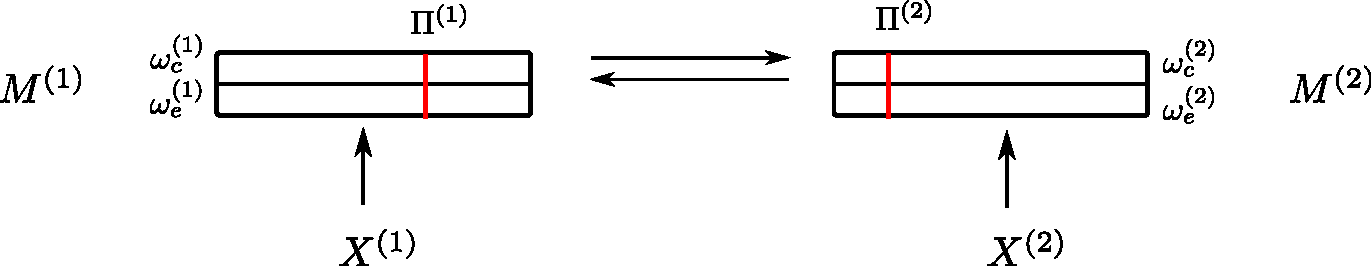
\includegraphics[width=\textwidth]{archi_2maps.pdf}
	\caption{Schéma de l'architecture de deux carte. Chaque carte possède une couche de poids externe $\w_e$ et une couche de poids contextuels $\w_c$. Les connexions sont rétroactives~: l'entrée contextuelle de $M\m{1}$ est la position du BMU de la carte $M\m{2}$ et inversement. 
	Chaque carte prend une entrée externe $\inpx$.\label{fig:archis}}
\end{figure}

\subsection{Modèles d'entrée et architecture de cartes}

Le modèle d'architecture que nous utilisons est présenté en figure~\ref{fig:archis}.
Chaque carte a une taille fixée de 500 n\oe{}uds, indexés entre 0 et 1, et possède deux couches de poids $\w_e$ et $\w_c$. 
Les rayons de voisinage sont fixés à $r_e = 0.2$ et $r_c = 0.02$, sauf si précisé autrement dans l'expérience.
Les connexions sont réciproques~: $M\m{1}$ prend comme entrée contextuelle $\bmu\m{2}$ et inversement.

Rappelons la définition des entrées multimodales~: il s'agit d'un ensemble d'entrées $\mathbf{\inpx} = (\inpx\m{1}, \cdots, \inpx\m{D})$.
Nous représentons la dépendance entre entrées en choisissant une variable latente du modèle, $U$, telle que~:
$$ \forall i, \inpx\m{i} = f\m{i}(U) + \epsilon\m{i}$$
avec $\epsilon\m{i}$ un bruit éventuel sur les entrées.
La dimension de $U$ détermine le degré de dépendance entre les entrées.
Dans tous les modèles, $U$ sera une valeur dans $[0,1]$.

Dans cette série d'expériences, nous comparons la réponse de l'architecture à différents modèles d'entrées.
Nous reviendrons d'abord sur le modèle du cercle \textbf{A}, qui a déjà été présenté au chapitre \ref{chap:repr}. L'intérêt d'utiliser cette courbe est que la disposition est symétrique~: toute entrée $X^{(1)}$ correspond à deux valeurs possibles pour $X^{(2)}$ et inversement. $U$ est dans ce cas une variable 1D correspondant à l'angle du point sur le cercle.
Nous comparerons ensuite les observations réalisées sur le modèle du cercle sur d'autres dispositions d'entrées, représentées en figure~\ref{fig:input_list}~:
\begin{itemize}
	\item Les entrées sont identiques \textbf{C}.
	\item Une entrée est une fonction de l'autre~: $\inpx\m{2} = cos(\inpx\m{1})$~\textbf{B}.
	\item Les entrées sont sur une courbe plus complexe que le cercle, ici une courbe de Lissajous \textbf{D}~: une entrée $\inpx\m{1}$ correspond à 4 à 6 valeurs de $\inpx\m{2}$ et inversement. $U$ est une variable 1D paramétrant la courbe.
	\item Les entrées sont totalement indépendantes, prises aléatoirement dans le carré $[0,1]^2$~\textbf{E}. $U$ est alors une variable 2D.
	\item Les entrées sont sur un anneau \textbf{F}. $U$ est alors une variable 1D, correspondant à l'angle du point sur le cercle, mais avec du bruit ajouté dans le modèle d'entrées. 
	Une carte de Kohonen classique a comme propriété d'être résistante au bruit sur les données. Ainsi, une carte 1D se dépliant sur un anneau fin en 2D apprendra d'abord une représentation du cercle sous-jacent. Nous voulons vérifier comment cette propriété se vérifie sur l'apprentissage de données par plusieurs cartes.
\end{itemize}

\begin{figure}[h!]
	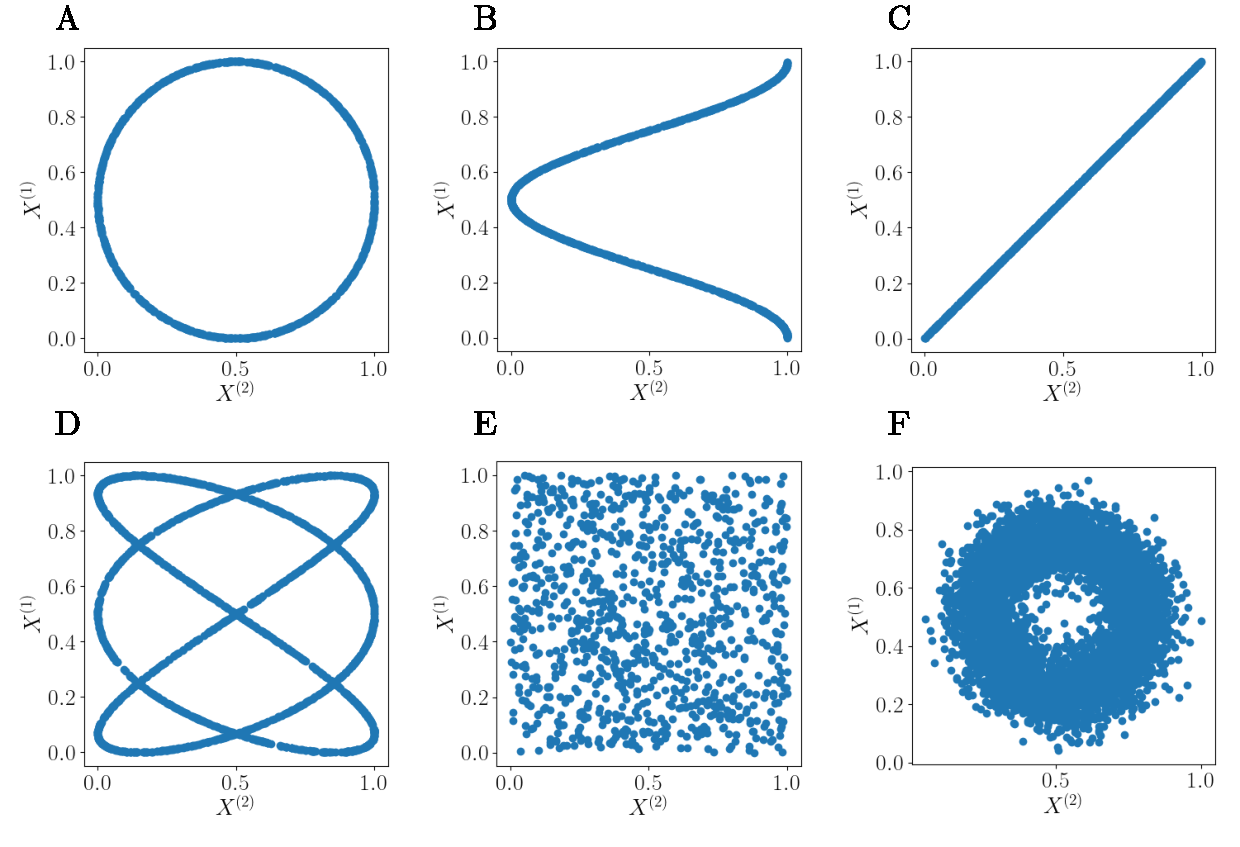
\includegraphics[width=\textwidth]{inputs/inputs.pdf}
	\caption{Dispositions d'entrées en deux dimensions utilisées dans cette section. $M\m{1}$ prend en entrée les valeurs $\inpx\m{1}$ et $M\m{2}$ les valeurs $\inpx\m{2}$. \label{fig:input_list}}
\end{figure}

Pour générer ces entrées, $U$ est tiré uniformément dans $[0,1]$, et un couple d'entrées $(\inpx\m{1},\inpx\m{2})$ généré à partir de la même valeur de $U$ sera toujours présenté à l'architecture lors de la même itération.
Lors de chaque expérience, nous réalisons l'apprentissage sur un échantillon de 20000 points, générés aléatoirement et présentés une fois à l'architecture. Les tests sont ensuite réalisés sur 1000 points générés aléatoirement selon la même distribution d'entrées que l'apprentissage.
Le code utilisé pour générer les expériences et les représentations est disponible en ligne.\footnote{\url{todo.github.com}}

\subsection{Observations réalisées sur le modèle d'entrées en cercle}

Revenons d'abord sur l'expérience sur le cercle \textbf{A}, déjà présentée au chapitre \ref{chap:repr}. 
Après avoir vérifié que les poids des cartes convergent bien au cours de l'apprentissage, nous détaillerons la disposition finale des poids externes et contextuels et la réponse de la carte, afin d'identifier des mécanismes traduisant l'apprentissage des entrées et des relations.

\subsubsection{Convergence des poids}

Dans une carte de Kohonen classique, le rayon de voisinage et le taux d'apprentissage sont diminués de façon prédéfinie au cours des itérations d'apprentissage.
Cette opération permet d'assurer un dépliement des cartes au début de l'apprentissage puis assure la convergence des poids $\w$ des cartes lorsque les paramètres sont faibles.
Dans notre étude, nous avons au contraire choisi de ne pas modifier les paramètres d'apprentissage au cours des itérations, comme expliqué en section~\ref{sec:parametres_carte} p.\pageref{sec:parametres_carte}.
Avant de s'intéresser à l'organisation après apprentissage, nous voulons donc vérifier que les poids des cartes convergent vers une position stable au cours de l'apprentissage.
Nous illustrons cette convergence en figure~\ref{fig:conv}, qui présente l'évolution des variations des poids $\w\ext$ et $\w\cont$ dans chaque carte au cours de l'apprentissage. 
Toutes les 100 itérations, nous calculons la moyenne sur les positions $p$ des différences entre $\w_t(p)$ et $w_{t-100}(p)$, pour chaque couche de poids~:
$$ \langle | \w_t(p) - w_{t-100}(p)| \rangle $$

Cette valeur a été calculée sur 10 apprentissages séparés, réalisés sur la même architecture, les mêmes distributions d'entrées, mais des échantillons d'entrées différents. Nous représentons sur la figure la valeur moyenne et l'écart type de cette différence sur les 10 expériences.
Nous pouvons constater que les poids évoluent rapidement au début de l'apprentissage, puis n'évoluent ensuite que très faiblement~: à l'itération 10000, chaque prototype $\w_e(p)$ se déplace en moyenne de 0.05 tous les 100 itérations, et chaque $\w_c(p)$ de 0.005.
Notons que ces tracés ne permettent pas de montrer expérimentalement une convergence des poids, mais donnent une bonne idée de l'évolution générale des poids des cartes. 
Graphiquement, nous avons observé que les poids évoluent vers une position stable.

Nous pouvons proposer des éléments d'explication de cette convergence observée empiriquement, en remarquant qu'une carte se comporte principalement comme une carte de Kohonen classique apprenant sur les entrées externes. En effet, l'activité externe domine dans le calcul de l'activité globale, cf. équation~\ref{eq:global_act}.
L'activité contextuelle est utilisée ici comme un terme de modulation d'amplitude de l'activité externe.
La convergence des poids d'une carte de Kohonen classique en 1D sur des données numériques a été démontrée, voir~\cite{cottrell_theoretical_2016}. 
On peut donc raisonnablement envisager que les poids des cartes CxSOM convergent également, pour des cartes 1D.
La convergence en l'absence de décroissance de paramètres pourra cependant poser plus de problèmes sur des cartes en deux dimensions.

\begin{figure}[ht]
	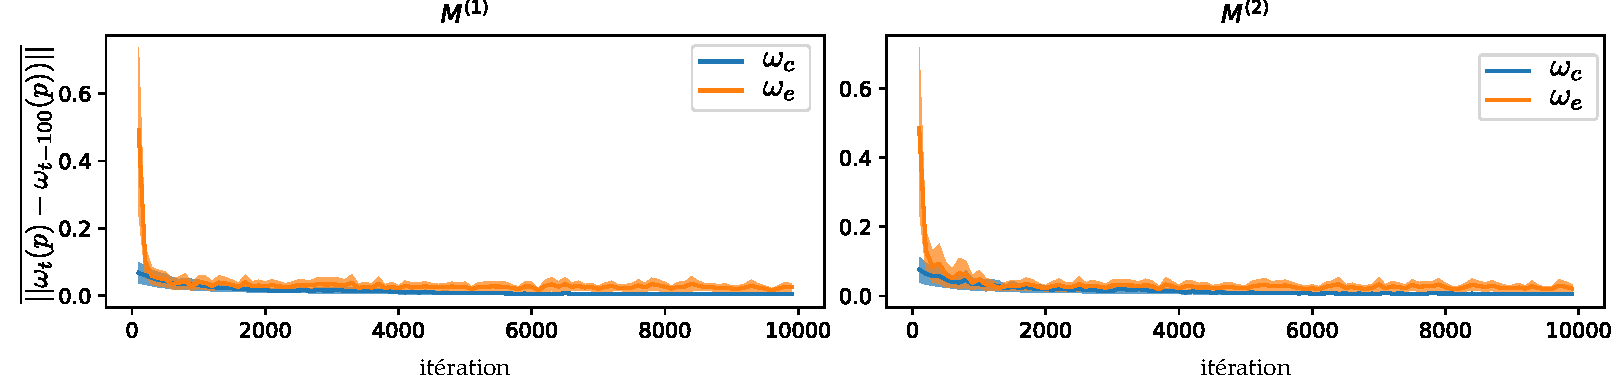
\includegraphics[width=\textwidth]{convergence/cercle_moy_2.pdf}
	\vspace{-0.5cm}
	\caption{Pour chaque carte, nous représentons l'évolution en fonction du temps d'apprentissage de la différence moyenne entre les poids d'une carte à l'instant $t$ et ceux à $t-100$, $\langle|\w_t(p) - \w_{t-100}|\rangle$.
	L'évolution est moyennée sur 10 apprentissages dont les entrées sont tirées aléatoirement selon la même distribution d'entrées (\textbf{(A)}).
	Ces tracés montrent que les poids externes et contextuels évoluent rapidement vers une position dans laquelle ils ne varient plus que faiblement.\label{fig:conv}}
\end{figure}


\subsubsection{Organisation des cartes après apprentissage}

Maintenant que nous avons observé que les poids convergent vers une organisation stable, nous voulons identifier comment les réponses et l'organisation des cartes de l'architecture traduisent un apprentissage du modèle d'entrée \textbf{A}.
Nous avions déjà présenté les méthodes de représentation et comparé la réponse de CxSOM à celle d'une carte simple au chapitre~\ref{chap:repr}.
Nous revenons ici sur ces observations en les complétant.

Reprenons les tracés introduits en figure~\ref{fig:inputs}, qui permettent d'observer les poids des cartes et d'associer les valeurs d'entrées à leur position de BMU.
Cette représentation est tracée pour les deux cartes de l'architecture en figures~\ref{fig:w} et \ref{fig:w_zoom}.
Les poids externes, en bleu, présentent une disposition similaire à ceux observés dans une carte classique~: ils sont classés de façon monotone entre 0 et 1. Les poids contextuels, en orange, présentent une forme de \og vagues \fg{}. En rouge et vert, nous y ajoutons la valeur des entrées $\inpx\m{1}$ et $\inpx\m{2}$ en fonction des positions de BMUs obtenues lors de la phase de test.

Nous observons que les positions des BMUs dans la carte $M\m{1}$ se répartissent en groupes, séparés par des zones mortes de la carte dont les n\oe{}uds n'ont jamais été BMUs. 
C'est une première différence avec une carte classique, pour laquelle toutes les positions seront BMUs lorsque les entrées sont distribuées de façon continue. 
Les zones dans lesquelles les n\oe{}uds sont BMUs correspondent aux extrema des poids contextuels et leurs alentours.

\begin{figure}[ht]
	\centering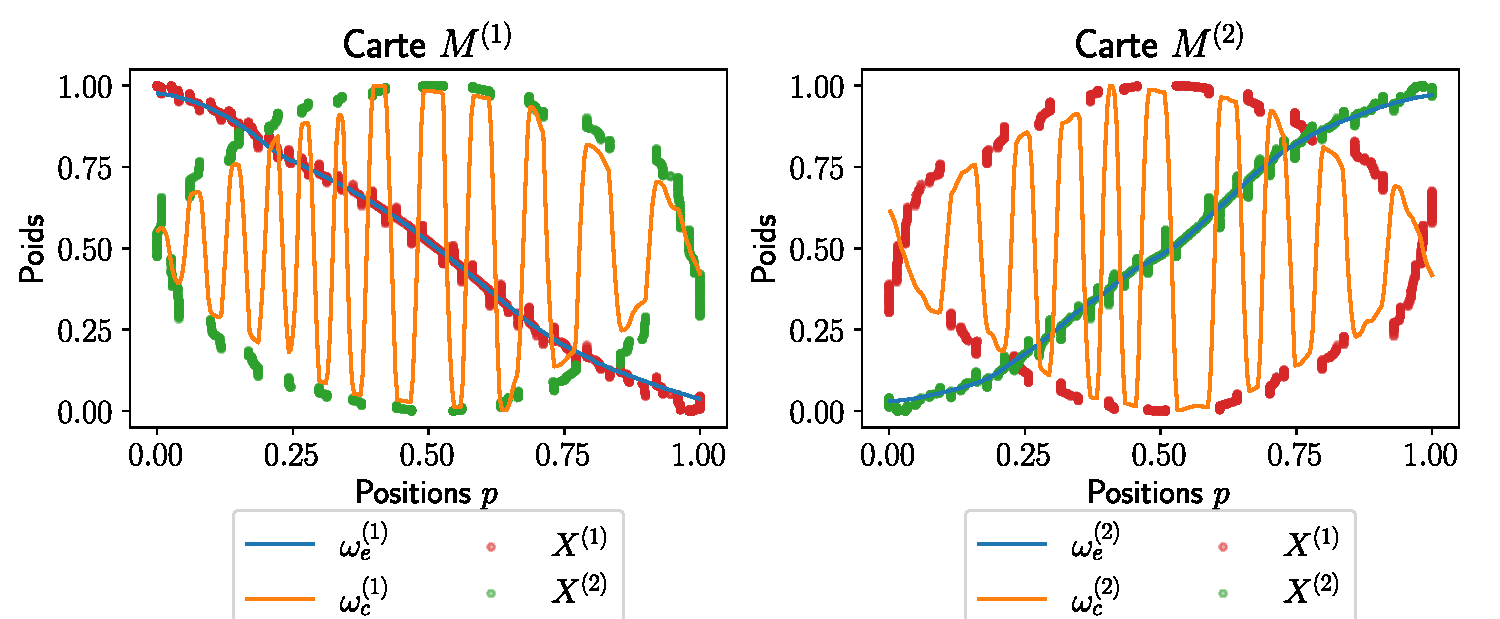
\includegraphics[width=\textwidth]{cercle/weights_500.pdf}
	\caption{Représentation cartographique des poids et entrées lors d'une phase de test selon la position du BMU dans chacune des cartes. Nous remarquons que les poids d'une carte, par exemple la carte $M^{(1)}$, s'organisent en zones différenciant les valeurs de la paire $X^{(1)}, X^{(2)}$ et non seulement la valeur de $X^{(1)}$. 
	Deux zones adjacentes codent pour des valeurs de $X^{(1)}$ proches, mais $X^{(2)}$ différents. 
	Au sein d'une même zone, les BMUs s'organisent sous la forme d'une sous-carte sur les valeurs de l'entrée contextuelle. Ces zones se forment de manière auto-organisée. \label{fig:w}}
\end{figure}

La figure~\ref{fig:w_zoom} est un agrandissement du tracé sur quatre zones de la carte $M\m{1}$.
Elle met en évidence le fait que les zones définies par les poids contextuels se partagent les positions des BMUs en fonction de la valeur de l'entrée contextuelle~:
Les deux points représentés en rouge et bleu ont la même valeur de $\inpx\m{1}$, mais une valeur différente de $\inpx\m{2}$. 
Ils ont ici un BMU différent dans la carte $M\m{1}$, situés dans deux zones adjacentes.
Les n\oe{}uds de deux zones adjacentes sont ainsi des BMUs pour des segments de valeur d'entrée externe qui se recouvrent.

\begin{figure}[ht]
	\centering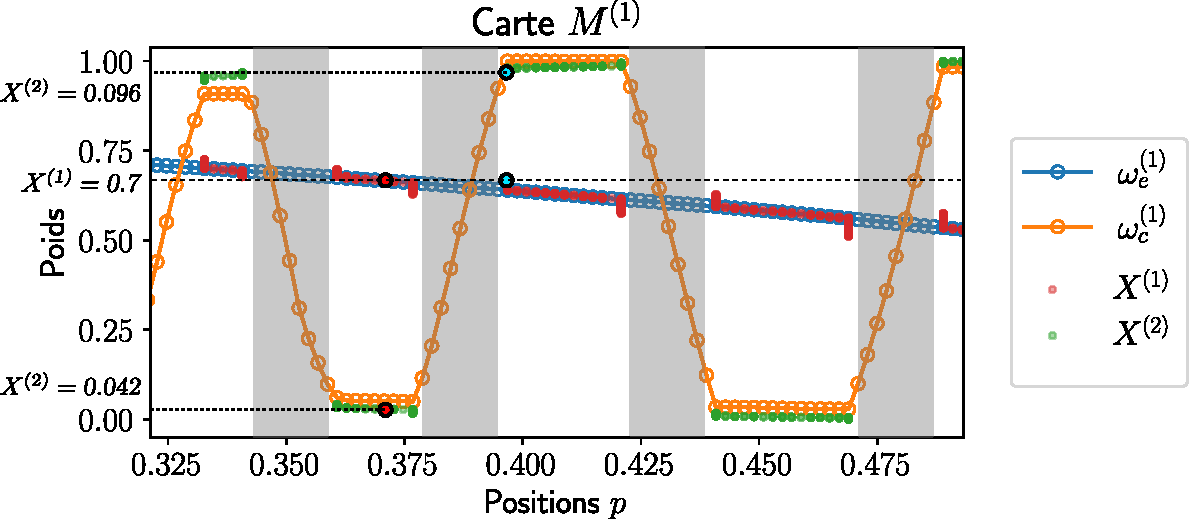
\includegraphics[width=0.7\textwidth]{cercle/weights_zoom_500.pdf}
   \caption{Zoom sur la figure \ref{fig:w} entre les positions 0.35 et 0.55 de la carte $M\m{1}$. 
   Nous y faisons apparaître la position sur la courbe des n\oe{}uds de la carte.
   Deux zones consécutives seront BMUs pour des ensembles d'entrées qui se recouvrent. Par exemple, les deux entrées correspondant aux points bleu et rouge ont les mêmes valeurs de $\inpx\m{1}$, mais des valeurs différentes de $\inpx\m{2}$. Leurs BMUs sont alors séparés dans la carte $M\m{1}$ dans deux zones consécutives.
   Entre les zones, quelques unités ne sont jamais BMU, en gris sur la figure. Il s'agit de zones mortes, créant des discontinuités dans la réponse de la carte.
   \label{fig:w_zoom}}
\end{figure}

Ces observations suggèrent que dans chaque carte, une position se spécialise en tant que BMU par rapport à son entrée externe et à son entrée contextuelle. 
Les cartes présentent une organisation à deux échelles, l'une relative à l'entrée externe, définissant les zones, et l'autre relative à l'entrée contextuelle.
% Ces zones sont créées par auto-organisation~; aucun paramètre de la carte n'a été modifié pendant l'apprentissage pour former ces zones.

\subsubsection{Erreur de quantification vectorielle}

Nous nous intéressons enfin à la quantification vectorielle réalisée par la couche de poids externe sur l'entrée externe dans chaque carte. 
Nous souhaitons que le poids externe du BMU soit une approximation de l'entrée externe, ce qui apporte une possibilité de reconstruction de l'entrée à partir du BMU.

La Figure~\ref{fig:qv} présente la valeur de cette approximation au sein de chaque carte, c'est-à-dire $\w\ext(\bmu\m{i})$, en fonction de l'entrée correspondante $\inpx\m{i}$. 
Cette figure montre que la quantification vectorielle est bien réalisée~: les valeurs approximées sont proches des valeurs d'entrées.
L'erreur de quantification est néanmoins plus importante que celle qu'on obtiendrait avec une carte de même taille et mêmes paramètres apprenant sur l'ensemble des $\inpx\m{i}$. Il s'agit d'un compromis réalisé par la carte pour pouvoir à la fois encoder son l'entrée externe et son entrée contextuelle en une seule position de BMU.
Nous remarquons enfin une disposition en étages, dus aux zones formées par les poids contextuels.
En effet, une même valeur d'entrée peut avoir un BMU dans deux zones de la carte, en fonction de la valeur de l'entrée contextuelle. 
Comme les poids externes sont strictement croissants ou décroissants, cela induit l'erreur observée dans la prédiction d'entrée.

\begin{figure}[h!]
	\centering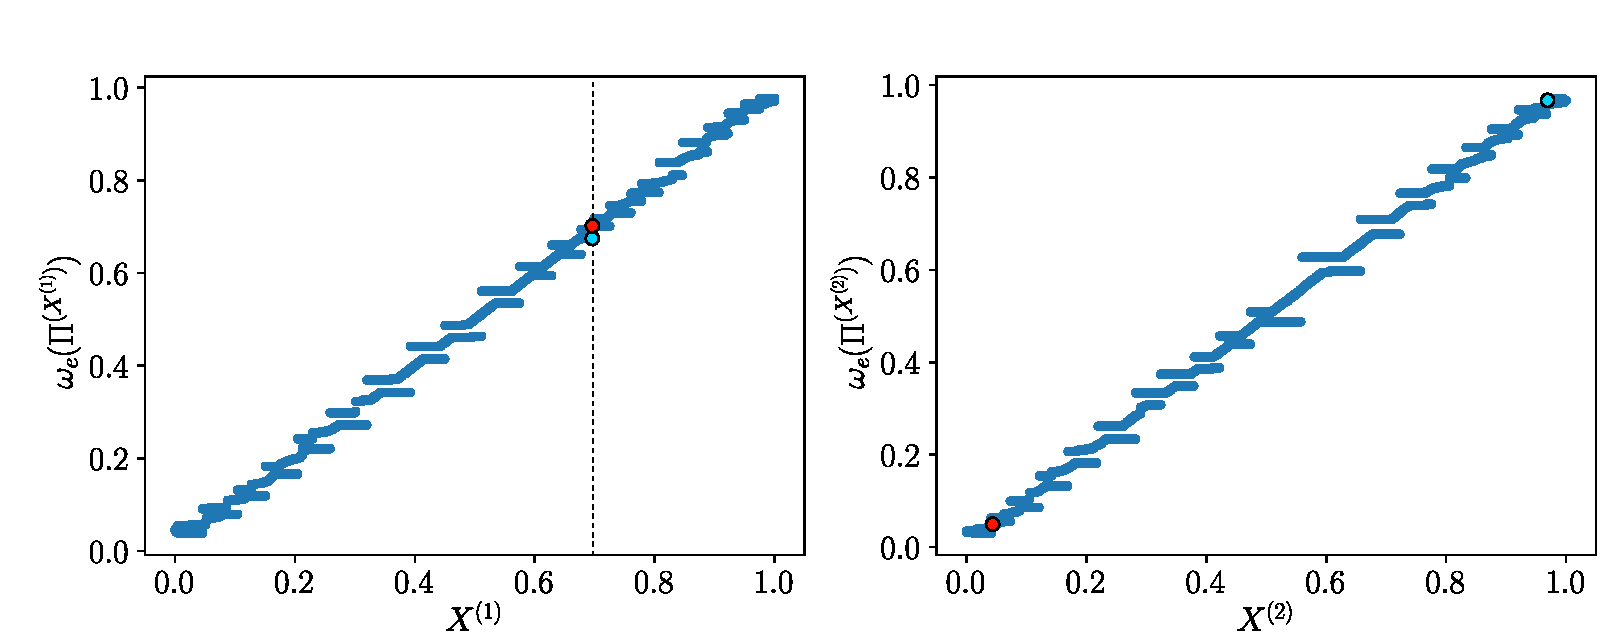
\includegraphics[width=\textwidth]{cercle/frz-error-500.pdf}
	\caption{Représentation de l'erreur de quantification sur les valeurs de $X^{(1)}$ et $X^{(2)}$. Le poids externe du BMU est proche de la valeur de l'entrée~; chaque carte réalise ainsi une bonne quantification vectorielle sur ses entrées. 
	Les poids rouges et bleus représentés en figure \ref{fig:w_zoom} sont reportés sur le graphique. \label{fig:qv}}
\end{figure}

\subsubsection{Apprentissage du modèle d'entrée par chaque carte}

En section~\ref{sec:u_bmu}, nous avons observé que l'apprentissage des relations entre entrées se traduit par une relation fonctionnelle entre $U$ et $\bmu$ dans chaque carte, tracée en figure~\ref{fig:piu}.
Cette propriété traduit l'observation qu'un BMU se spécialise en fonction de l'entrée externe et des entrées contextuelles, qui a également été mise en valeur par la représentation cartographique au paragraphe précédent. Nous reviendrons plus en détail sur cette représentation et la propriété de relation fonctionnelle entre la variable cachée et la position du BMU au chapitre~\ref{chap:indicateur}.

\subsubsection{Résumé des observations}

Les résultats de cette expérience ainsi que les observations présentées au chapitre~\ref{chap:repr} nous permettent de formuler les hypothèses suivantes concernant les comportements élémentaires d'apprentissage d'une architecture de deux cartes 1D~:

\begin{itemize}
	\item Les poids externes de chaque carte de l'architecture permettent d'effectuer une bonne quantification vectorielle de ses entrées externes.
	\item Les poids contextuels de chaque carte définissent des zones distinctes de BMU. 
	Chaque zone réagira à un même intervalle de valeur pour à la fois l'entrée externe et l'entrée contextuelle. Deux zones adjacentes encodent des valeurs d'entrée externe proches, mais des valeurs distinctes d'entrée contextuelle.
	Entre chaque zone de BMUs, nous observons des zones mortes dans lesquelles les n\oe{}uds ne sont jamais BMUs. Ce comportement en zones forme deux échelles de quantification.
	\item L'apprentissage du modèle d'entrée par l'architecture se traduit par l'existence d'une relation fonctionnelle entre $U$ et $\bmu$ dans chaque carte, montrant que chaque carte encode le modèle d'entrée complet et non seulement son entrée externe.
\end{itemize}

Nous cherchons dans la suite de ce chapitre à vérifier ces hypothèses sur les autres dispositions d'entrées en deux dimensions, et à compléter les observations.
Nous étudierons en particulier comment les zones se forment et quelles propriétés d'apprentissage elles confèrent à l'architecture de cartes.
Nous verrons ensuite en section \ref{sec:pred} que la formation de ces zones ainsi que la propriété de quantification vectorielle de l'entrée externe permet à l'architecture de cartes de prédire des entrées manquantes lors d'une phase de test.

\subsection{\'Evaluation de l'organisation sur les autres distributions d'entrées}

Nous reprenons les dispositions d'entrées \textbf{B},\textbf{C},\textbf{D},\textbf{E}.
Dans toutes ces dispositions, nous avons vérifié que la quantification vectorielle est bien réalisée dans chaque carte sur ses entrées, que nous n'avons pas tracée ici.
Nous nous concentrerons sur la présence ou non de zones de poids contextuels dans l'organisation finale des poids en fonction de la distribution des entrées.

Dans la disposition d'entrées \textbf{C}, une valeur de $\inpx\m{1}$ correspond à une seule valeur de $\inpx\m{2}$ dans le modèle. 
Nous nous attendons à ce que l'architecture de cartes n'aie pas besoin de séparer les BMUs en zones.
La figure \ref{fig:id_results} présente la disposition des poids et entrées des cartes résultant de l'apprentissage. 
Dans ce cas, les poids externes et contextuels ne forment effectivement pas de zones, ce qui est bien ce que nous attendions.
En figure~\ref{fig:cos_results}, la dépendance entre les entrées n'est plus bijective~: $\inpx\m{2}$ est toujours fonction de $\inpx\m{1}$, mais pas l'inverse (Entrées \textbf{B}). 
Nous observons que la carte $M\m{1}$ ne forme pas de zones, car une seule valeur de $\inpx\m{2}$ correspond à une même valeur de $\inpx\m{1}$, ce qui est cohérent avec le comportement sur les entrées identiques.
Au contraire, la carte $M\m{2}$ doit à présent se diviser pour apprendre les deux valeurs de $\bmu\m{1}$ possibles correspondant à $\inpx\m{2}$. Ce comportement rejoint ainsi celui que nous avons observé sur le cercle.
D'après ces deux expériences, la formation de zones semble ainsi intervenir seulement lorsqu'une carte $i$ doit séparer deux points différents dans le modèle d'entrée, mais partageant une même valeur sur la modalité $\inpx\m{i}$.


\begin{figure}[H]
	\centering\includegraphics[width=0.8\textwidth]{id/weights.pdf}
	\vspace{-0.3cm}
	\caption{Représentation cartographique des poids et entrées pour la disposition identité \textbf{C}. Les poids externes et contextuels sont superposés, et les poids contextuels n'ont pas besoin de former de zones. \label{fig:id_results}}
\end{figure}


\begin{figure}[H]
	\centering\includegraphics[width=0.8\textwidth]{cos/weights.pdf}
	\vspace{-0.3cm}
\caption{Représentation cartographique des poids et entrées pour $\inpx\m{2} = cos(\inpx\m{1}$ \textbf{B}. Les poids contextuels de la carte $M\m{1}$ ne forment pas de zones car une valeur de $\inpx\m{1}$ correspond toujours à une seule valeur de $\inpx\m{2}$. Au contraire, les poids de la carte $M\m{2}$ s'organisent pour gérer une distinction~: pour une même valeur de $\inpx\m{2}$, deux $\inpx\m{1}$ sont possibles. \label{fig:cos_results}}
\end{figure}
\begin{figure}[H]
	\centering\includegraphics[width=0.8\textwidth]{lissa/weights.pdf}
	\vspace{-0.3cm}
	\caption{Représentation cartographique des poids et entrées pour des entrées sur une courbe de Lissajous, \textbf{D}.
	Les poids contextuels se disposent toujours en zones afin de différencier les BMUs selon l'entrée externe et l'entrée contextuelle.
	Une zone est une carte organisée d'une sous-région des entrées externes. \label{fig:lissa}}
\end{figure}

\begin{figure}[H]
	\centering\includegraphics[width=0.8\textwidth]{square/weights.pdf}
	%\vspace{-0.5cm}
	\caption{Représentation cartographique des poids et entrées dans le patch $[0,1]^2$, \textbf{E}. Les poids contextuels s'organisent en zones qui forment une carte organisée des sous-régions de l'espace d'entrée externe. \label{fig:ind}}
\end{figure}

Regardons maintenant l'organisation des cartes lorsqu'une valeur de $\inpx\m{1}$ correspond à plus de deux valeurs de $\inpx\m{2}$~: 4 valeurs dans le cas de la courbe de Lissajous (Entrées \textbf{D}) ou tout l'intervalle $[0,1]$ dans le cas du patch $[0,1]^2$ (Entrées \textbf{E}). 
Ces organisations sont tracées en figure~\ref{fig:lissa} et \ref{fig:ind}.
Dans ces deux derniers cas, les cartes présentent encore une organisation en zones des poids contextuels.
Le nombre de zones est similaire à ce qui est observé sur le cercle, alors que la répartition des entrées est différente. 
Par contre, la forme des zones varie légèrement par rapport aux observations précédentes.
Nous observons en figure \ref{fig:ind} qu'une zone de BMUs dans $M\m{1}$ agit comme une \og sous-carte \fg de toutes les valeurs possible de l'entrée $\inpx\m{2}$ correspondant à un même intervalle de l'entrée  $\inpx\m{1}$.


Nous pouvons conclure de ces expériences que la présence de zones est un comportement systématique de la carte étant donné qu'elles sont observées même lorsque les entrées sont indépendantes.
Cependant, elles émergent de l'organisation seulement lorsqu'elles sont nécessaires~: lorsque la carte doit pouvoir différencier au moins deux points différents du modèle  d'entrée correspondant à une même valeur d'entrée externe.
La forme des zones et la réponse des cartes dépend ensuite de la relation entre les entrées.
Ainsi, sur la distribution {\textbf{E}}, la carte ne présente pas de zone morte. 
La totalité de chaque zone se déploie de manière à couvrir l'ensemble des valeurs $[0,1]$ d'entrée contextuelle. En effet, dans ce modèle d'entrée, une même valeur de $\inpx\m{1}$ correspond bien à tout l'intervalle $[0,1]$ pour $\inpx\m{2}$, et inversement.
Ce même comportement est également observé en figure ~\ref{fig:lissa} pour les courbes de Lissajous.
Une zone agit finalement comme une carte organisée des entrées contextuelles correspondant à d'une sous-région de l'espace d'entrée. 
Sur le modèle d'entrée tirées sur le cercle \textbf{A}, les BMUs se concentrent autour des extrema des poids contextuels, car pour une zone, seulement deux valeurs d'entrée contextuelles sont possibles.
Ces zones se forment de manière auto-organisée au cours de l'apprentissage.

Intéressons-nous plus en détail à l'apprentissage de la représentation du modèle d'entrée dans le cas des entrées indépendantes \textbf{E}.
En figure~\ref{fig:2som_p_d}, nous traçons la distorsion des poids externes des cartes~: $(\omega_e(\bmu\m{1}))$ en fonction de  $\omega_e(\bmu\m{2}))$, et reliées selon l'ordre des connexions de $M\m{1}$ puis $M\m{2}$.
Ce tracé nous permet de visualiser la quantification vectorielle dans l'espace d'entrée multimodal et non seulement sur chaque carte. Nous y observons que les cartes quantifient tout l'espace $[0,1]^2$, mais que seulement 90 points sont définies par la quantification vectorielle, alors que les deux cartes sont de taille 500. 
Ces points sont définis par les zones de poids contextuels des cartes.
 Enfin, nous voulons vérifier si les cartes sont robustes au bruit en prenant des données en forme d'anneau (Entrées~\textbf{(F)}), représentées en figure~\ref{fig:anneau_w}. Nous nous attendons à un comportement similaire à celui observé sur le cercle, mais avec une marge de quantification un peu plus élevée, ce qui est bien le cas sur le tracé.

\begin{figure}[H]
	\hfill\begin{minipage}{0.4\textwidth}
		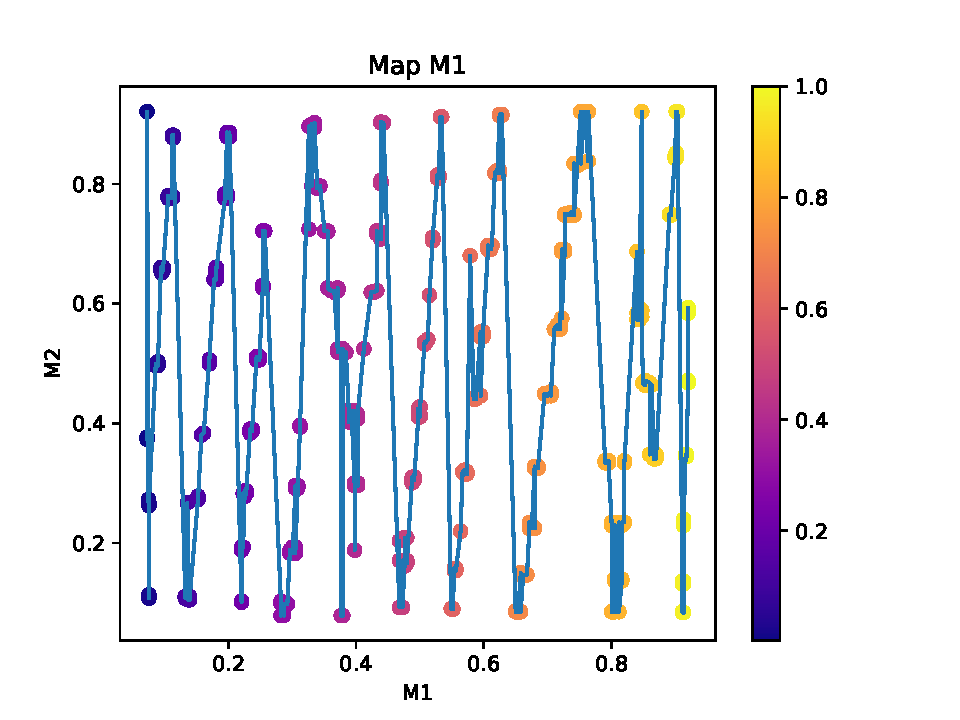
\includegraphics[width=\textwidth]{2som_square_d}
	\end{minipage}
	\begin{minipage}{0.4\textwidth}
		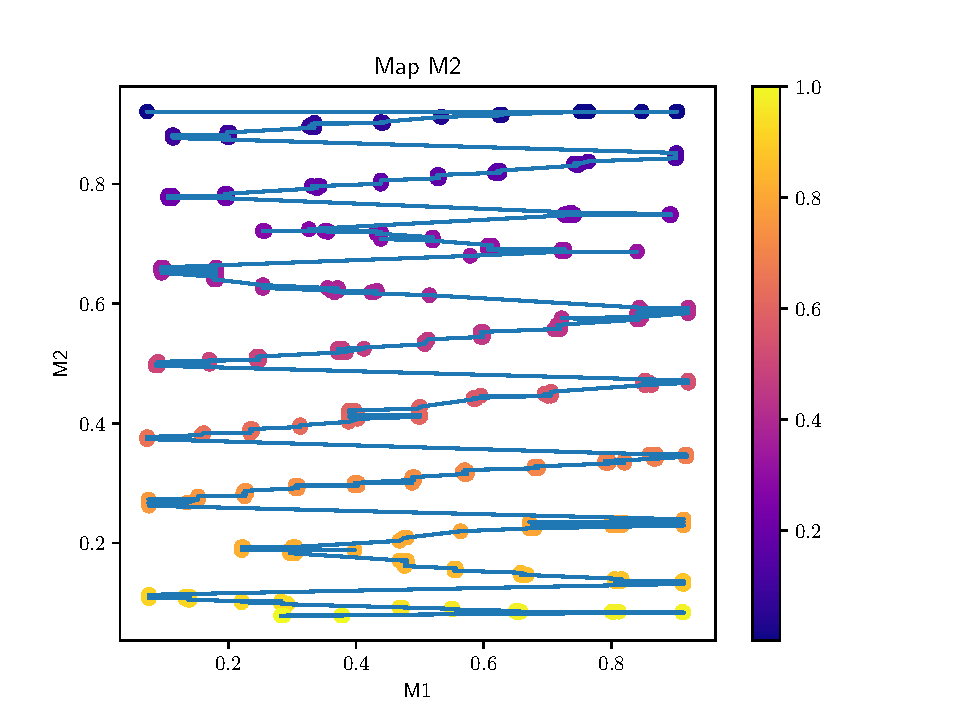
\includegraphics[width=\textwidth]{2som_square_d2}
	\end{minipage}\hfill
	\caption{Représentation de la distorsion des poids des deux cartes sur le modèle d'entrée \textbf{E}. Les cartes s'organisent de façon à représenter tout le patch $[0,1]^2$, l'une selon les $\inpx\m{1}$, l'autre selon les $\inpx\m{2}$. Bien que chaque carte aie 500 n\oe{}uds, on observe seulement environ 90 valeurs possibles des paires $\w_e(\bmu\m{1}),\w_e(\bmu\m{2})$ \label{fig:2som_p_d}}
\end{figure}

\begin{figure}[H]
	\centering\includegraphics[width=0.8\textwidth]{anneau/weights_001.pdf}
	\caption{Représentation cartographique des poids et entrées pour des entrées sur un anneau. La disposition des poids et la réponse des cartes est similaire à celle de l'architecture apprenant sur le cercle. Une architecture de cartes est robuste au bruit sur les entrées externes, ce qui étend les propriétés de robustesse au bruit d'une carte de Kohonen classique à CxSOM. \label{fig:anneau_w}}
\end{figure}


La dernière observation que nous avions relevé sur le cercle est que $U$ est une fonction de la position du BMU dans chaque carte, ce qui montre que chaque carte de l'architecture a appris une représentation du modèle d'entrée. Le tracé de $U$ selon $\bmu$ dans la disposition d'entrée en courbe de Lissajous est par exemple représenté en figure~\ref{fig:u_bmu_lissa}. 
Cette figure fait également apparaître $U$ comme une fonction de la position du BMU dans chaque carte, ce qui étend l'observation réalisée sur le cercle.
Nous reviendrons plus en détail sur l'utilisation de $U$ dans l'analyse des réponses des cartes au chapitre \ref{chap:indicateur}.

D'après ces observations, nous concluons que la formation de zones de BMUs grâce aux poids contextuels est une propriété d'organisation systématique d'une architecture de deux cartes CxSOM. Une position de BMU encode alors non seulement une entrée externe mais aussi l'entrée contextuelle grâce à une deuxième échelle d'indices dans la carte. Ces deux niveaux d'indexation se forment de façon auto-organisée, et seulement lorsqu'il est nécessaire de pouvoir distinguer plusieurs valeurs du modèle $U$ correspondant à la même entrée externe dans une carte.


\begin{figure}[t]
	\centering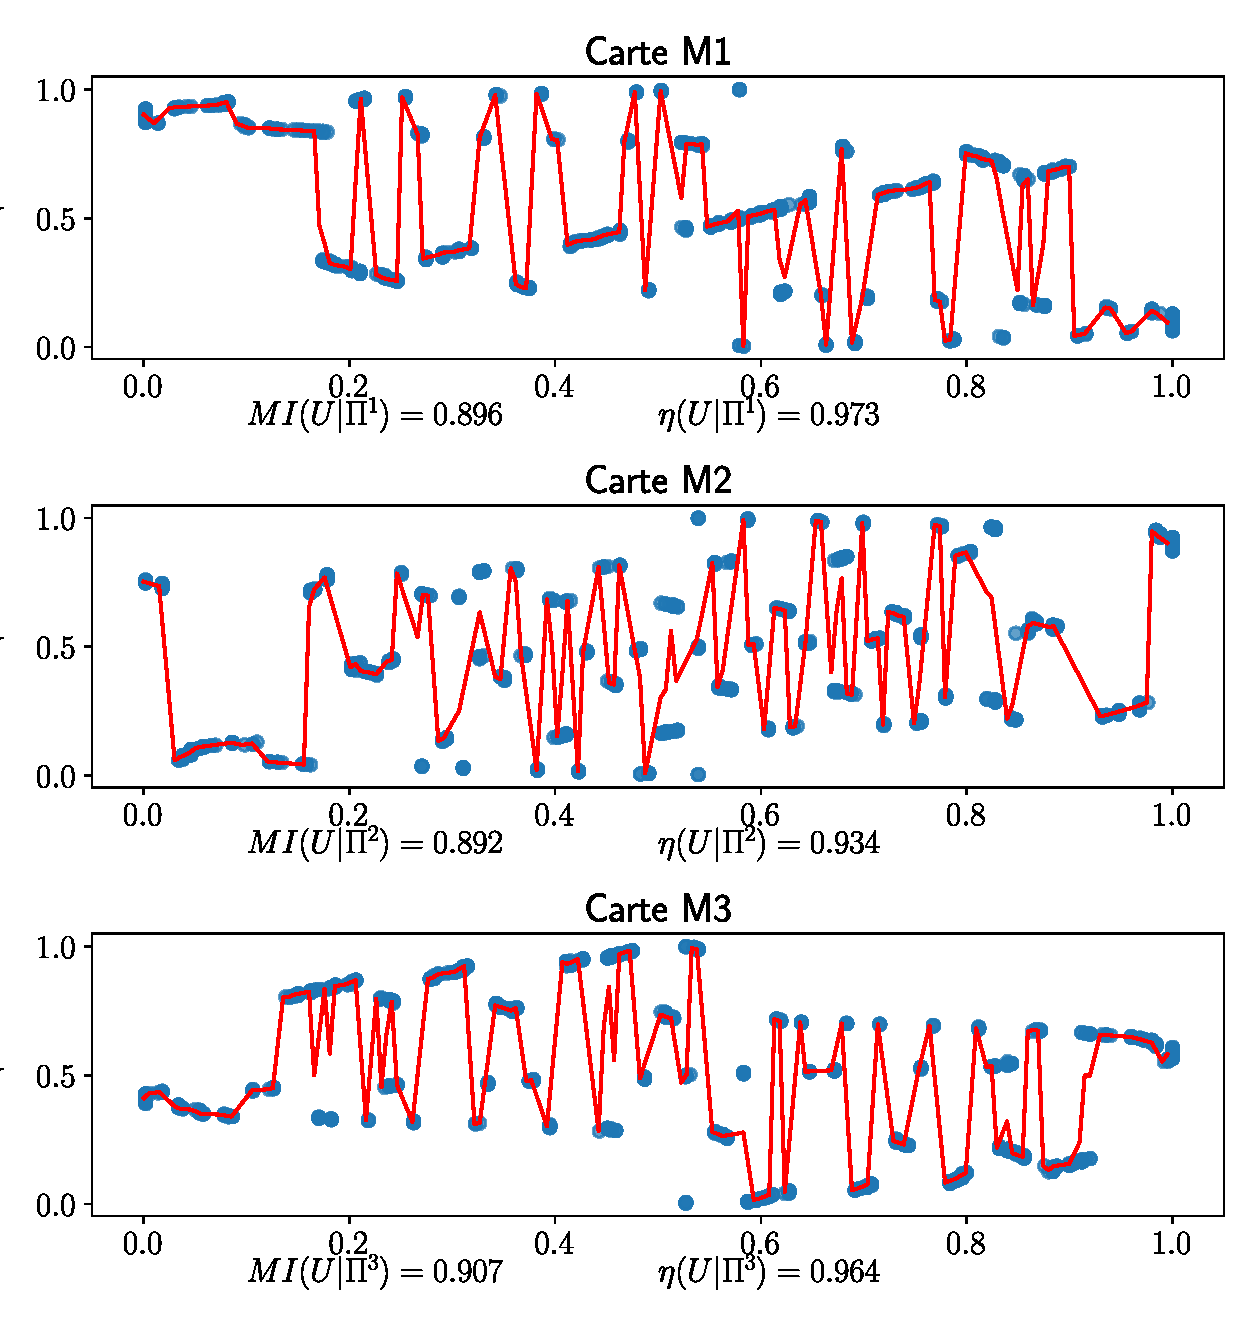
\includegraphics[width=0.8\textwidth]{lissa/U_BMU_19999.pdf}
	\caption{Représentation de $U$ selon le BMU $\bmu\m{i}$ dans chaque carte pour des entrées sur une courbe de Lissajous \textbf{D}. La courbe en rouge montre l'approximation du nuage de points par une fonction~: $U$ est ici une fonction de la position du BMU dans chaque carte, ce qui vérifie l'observation réalisée sur le cercle.\label{fig:u_bmu_lissa}}
\end{figure}

\subsection{\'Etude des mécanismes de formation des zones de poids contextuels}

L'organisation en zones observée sur les distributions d'entrées en 2D nous ont montré que les poids des cartes s'organisent en fonction de l'entrée externe, puis des zones se forment systématiquement pour différencier les différentes valeurs possibles du modèle d'entrée. Les zones se forment dès lors que plusieurs valeurs d'entrées contextuelles correspondent à une même valeur d'entrée externe dans une carte~: leur présence et la forme des poids contextuels dépend du modèle d'entrée.
L'organisation et le nombre de zones sont en revanche liées aux mécanismes d'apprentissage de la carte.
Nous nous intéressons maintenant aux paramètres des cartes influençant la formation de zones.
Nous avons observé que la présence de zones est liée en particulier aux rapports entre rayons de voisinage externes et contextuels.
Nous comparons dans cette section l'organisation obtenue sur plusieurs architectures ayant des couples de rayons de voisinage contextuels et externes différents, sur une même disposition d'entrée.

\subsubsection{Influence du rapport entre rayons de voisinage sur la formation de zones}

Nous reprenons les entrées \textbf{A}, en cercle et lançons l'apprentissage de plusieurs architectures dans lesquelles le rapport $\frac{r_e}{r_c}$ est différent.
Nous fixons $r_e$ à $0.2$ et faisons varier $r_c$ de $0.2$ à $0.005$.

En figure \ref{fig:rcre}, nous traçons la représentation cartographique de $M\m{1}$ après apprentissage pour ces différents rayons de voisinages.  Nous n'avons pas représenté $M\m{2}$, mais son comportement est semblable à $M\m{1}$ par la symétrie des entrées.
Pour $r_c = r_e$, ainsi que $r_c \geq r_e$, la carte ne s'organise pas en zones. 
La formation de celles-ci intervient pour $r_c < r_e$. Sur la figure, nous commençons à voir des zones de poids contextuels apparaître pour $r_e = 3r_c$, sans que les BMUs ne marquent de séparation claire. Les zones sont réellement marquées à partir de $r_e = 4r_c$.
Le nombre de zones de BMU augmente ensuite avec le rapport des rayons de voisinage. Plus il y a de zones, plus la quantification réalisée sur l'entrée externe est précise.
La taille du rayon de voisinage contextuel est ensuite limité par la taille de la carte. Si celui-ci est trop faible, la notion de zone de poids contextuel n'a plus lieu d'être. C'est ce qu'on observe pour $\frac{r_e}{r_c} = 40$. $r_c$ est alors de 0.005, soit $2$ n\oe{}uds, les cartes ayant 500 n\oe{}uds. 
Chaque zone de BMU ne contient en fait que quelques n\oe{}uds, on ne peut donc plus vraiment parler de sous-carte. Néanmoins, cette disposition sépare toujours les BMUs en fonction de l'entrée externe et contextuelle. 
Nous verrons dans la suite du chapitre que la disposition en zones est nécessaire pour permettre l'apprentissage des relations entre entrée. Les rayons de voisinage doivent être choisis de façon à permettre la formation de zones. 
Le choix des paramètres les plus adaptés à une application reste à déterminer dans les travaux futurs.

\begin{figure}[ht]
	\includegraphics[width=\textwidth]{rceqre/rcre_tot.pdf}
	\caption{Représentation cartographique de la carte $M\m{1}$ pour différents rayons de voisinage contextuels, le rayon de voisinage $r_e$ étant fixé à $0.2$. Nous observons que la présence de zones dépend du rapport entre les rayons de voisinage. La carte définit des zones de BMUs grâce à la forme poids contextuels, de plus en plus nombreuses et contenant de moins en moins d'unités lorsqu'on augmente le rapport entre rayons de voisinage.
	La carte $M\m{2}$, non représentée ici, se comporte de façon similaire.\label{fig:rcre}
	}
\end{figure}	

L'organisation au sein d'une zone et la forme des poids contextuels dépendent ensuite du modèle d'entrées.

Nous pouvons expliquer la formation des zones par le fait que le rapport entre rayons de voisinage introduit deux échelles d'élasticités dans les poids ainsi que deux échelles temporelles de mise à jour.
D'une part, les poids externes se déplient plus vite que les poids contextuels, car le grand rayon de voisinage externe permet de mettre à jour plus de prototypes à chaque itération.
D'autre part, les poids externes présentent une \og attraction \fg{} plus forte sur les unités voisines~· l'élasticité de la couche de poids externe est plus élevée.
Les poids contextuels doivent donc composer avec cette force, l'organisation des poids contextuels est ainsi subordonnée à l'organisation des poids externes.

Dans nos expériences, nous avons pris des $r_c$ identiques pour toutes les couches de poids contextuels.
Nous pourrions cependant associer à chaque couche de poids d'une carte un rayon de voisinage différent. 
Enfin, nous pouvons aussi faire varier le taux d'apprentissage $\alpha$, ainsi que les paramètres de la fonction d'activation $\beta$, $\sigma$, etc.
Pour pouvoir adapter ces paramètres automatiquement dans un objectif d'application et réaliser une étude paramétrique approfondie, il nous faudrait définir une fonction caractérisant l'organisation d'une carte ou relative à un objectif d'apprentissage. 
Nous discuterons d'un tel indicateur au chapitre \ref{chap:indicateur}, mais soulignons ici que nous n'avons pas encore défini de valeur adéquate. C'est pourquoi nous nous sommes intéressés à la compréhension de l'effet des paramètres dans nos travaux, et n'avons pas cherché à optimiser ces valeurs.

\subsubsection{Influence de la présence de zones sur la recherche de BMU par relaxation}

Nous avons vu que la formation de zones de poids contextuels dépend des paramètres de la carte, et qu'elles se forment de manière auto-organisées grâce aux règles d'apprentissage des cartes.
Nous nous interrogeons sur l'influence de cette disposition dans le processus de relaxation.
Nous pouvons en effet penser que ces zones favorisent la recherche de consensus lors de la relaxation et la convergence des poids, ce que nous voulons vérifier ici.
Pour cela, nous comparons les indicateurs d'évolution de la convergence de la relaxation, introduits au chapitre~\ref{chap:relaxation} sur deux expériences.
Nous reprenons d'une part l'organisation obtenue en section~\ref{sec:2som_cercle}, dans laquelle les poids contextuels ont formé des zones, que nous comparons à un apprentissage réalisé sur les mêmes entrées, mais dans laquelle les cartes n'ont pas formé de zones~: $\frac{r_e}{r_c} = 1$. 
Nous traçons en figure~\ref{fig:conv_rcre} les indicateurs de la convergence de la relaxation~: en haut, nous représentons l'évolution du nombre de pas moyens nécessaires à la relaxation sur une phase de test, pour des tests réalisés régulièrement au cours des 1000 premiers pas d'apprentissage.
En bas, nous traçons le pourcentage d'entrées ayant mené à une convergence de la relaxation au cours de ces mêmes phases de test, chaque phase de test contenant 1000 points.
Dans les deux cas, nous observons une évolution similaire de ces deux valeurs. Les phases de test en fin d'apprentissage convergent dans plus de 95 \% des cas, convergence qui s'effectue en moyenne en une dizaine de pas de relaxation.
La présence de zones n'apparaît donc pas favoriser la relaxation.
Cette observation suggère que la convergence de la relaxation n'est pas spécifiquement liée à la formation de zones dans une carte, donc aux rayons de voisinages.

\begin{figure}[hb]
	\centering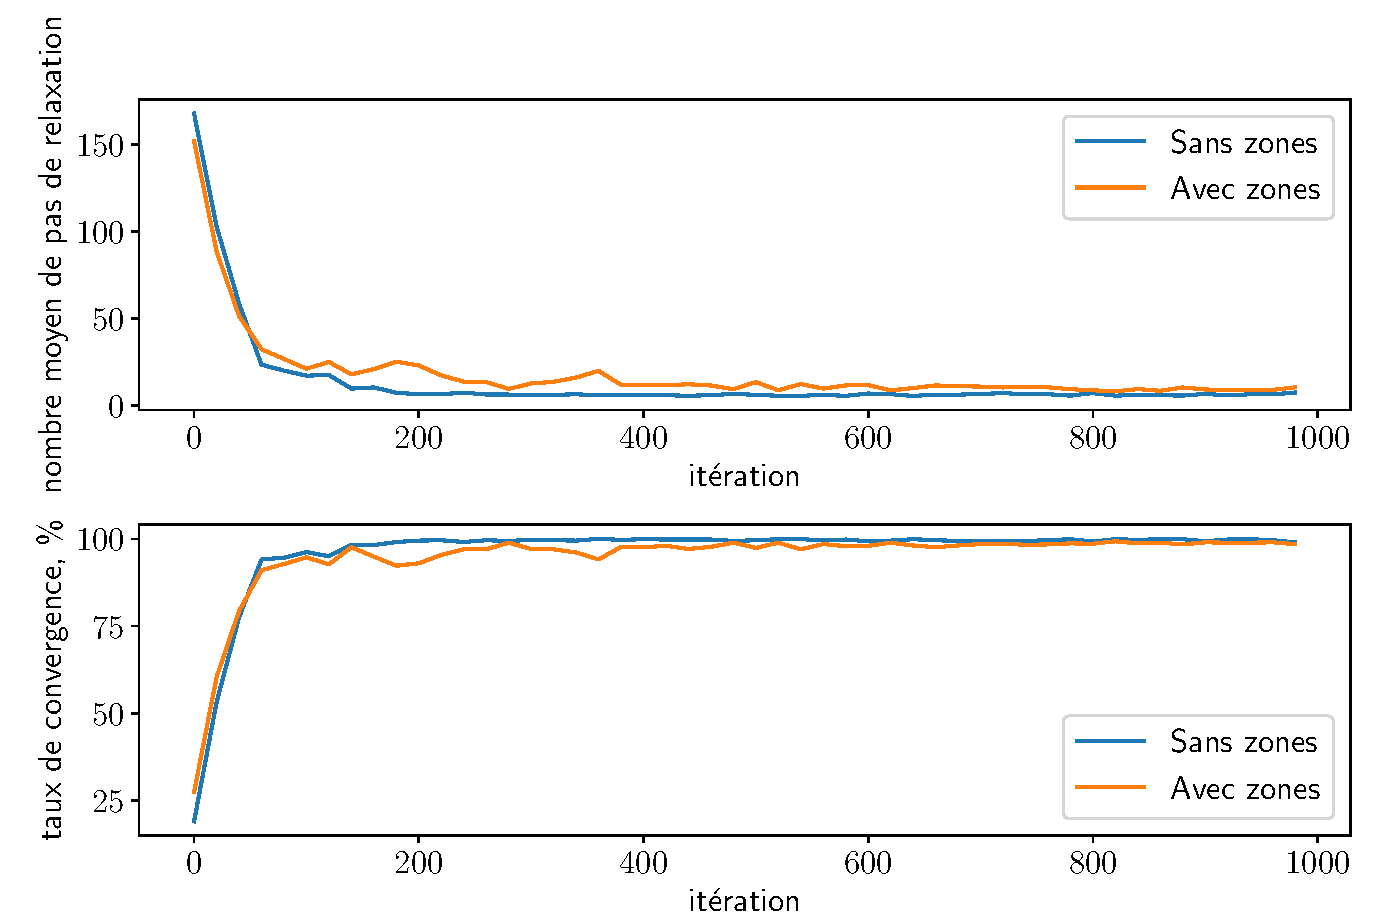
\includegraphics[width=0.8\textwidth]{rceqre/convergence_relax.pdf}
	\caption{\'Evolution du nombre moyen de pas de relaxation et du taux de convergence pour une organisation de cartes ayant formé des zones de poids contextuels ($\frac{r_e}{r_c} = 10$) et une organisation n'ayant pas formé de zones ($\frac{r_e}{r_c} = 1$). Dans les deux cas, la relaxation mène à un consensus en fin d'apprentissage. La formation de zones ne semble donc pas intervenir dans la qualité de la convergence de la relaxation. \label{fig:conv_rcre}}
\end{figure}

\subsection{Discussion}

Les motifs en zones formés par les poids contextuels sont un mécanisme qui émerge du processus d'évolution des cartes.
Le nombre de zones dépend des paramètres de l'architecture, puis l'organisation au sein des zones dépend ensuite de l'organisation des entrées. 
Au sein d'une même zone, les poids externes ont des valeurs très proches et les poids contextuels s'organisent de manière à former une sous-carte des valeurs possibles de l'entrée contextuelle pour un même intervalle de valeurs d'entrée externe.

On pourrait donc introduire une notion d'indices primaires et secondaires dans la carte, l'indice primaire étant celui de la zone et l'indice secondaire la position dans la zone.
Cette notion d'indices primaires et secondaires est observée en biologie dans le cerveau. 
Par exemple, la figure~\ref{fig:ballard} présente un schéma d'organisation des neurones du cortex V1 décrit en \cite{ballard_cortical_1986}.
Les auteurs observent que des neurones situés à différents emplacements sur le cortex visuel ne reçoivent pas la même partie du champ de vision, et leur emplacement correspond à la partie du champ de vision traitée (gauche - droite, etc).
Ces entrées différenciées forment une indexation~\emph{primaire} de V1. 
Au sein d'une zone de même indice primaire, les neurones s'organisent alors de façon à représenter tout le sous-espace des entrées ayant été présenté à la zone. Cette sous-carte définit alors des indices secondaires.
Dans CxSOM, la même entrée est certes présentée à toute la carte, donc la proximité avec ce modèle biologique est limitée. On peut quand même noter qu'après apprentissage, un n\oe{}ud de la carte ne réagit qu'à un sous-ensemble d'entrées définies par les valeurs des poids externes autour cet emplacement, ce qui se rapproche de ce phénomène de spécialisation d'une zone de neurones observé en biologie.

\begin{figure}[H]
	\centering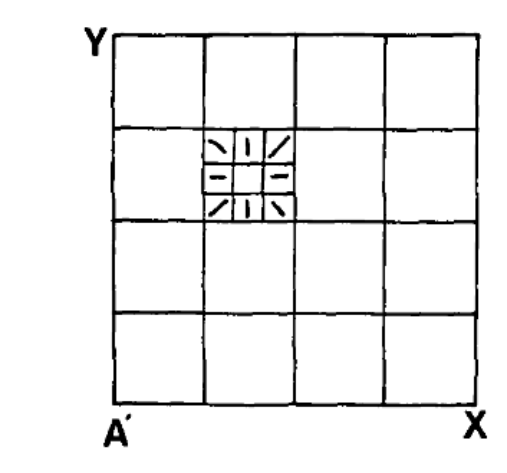
\includegraphics[width=0.3\textwidth]{ballard_primary_secondary.png}
	\vspace{-0.5cm}
	\caption{Schématisation d'une répartition en indices primaires et secondaire des neurones d'une aire corticale, tirée de~\cite{ballard_cortical_1986}. 
	Les auteurs observent que la réponse des neurones du cortex est organisée en zones selon leur position, formant des indices primaires. Les carrés de la figure représentent cette première indexation.
	Ces zones reçoivent différentes portions de l'espace d'entrée~: les zones situées à gauche du cortex traitent les signaux venant du champ visuel de gauche et ainsi de suite pour couvrir tout le champ visuel.
	Au sein d'une zone, les neurones cartographient toutes les valeurs possibles de l'entrée sous forme de carte topologiquement ordonnée, formant une indexation secondaire. \label{fig:ballard}}
\end{figure}

D'un point de vue du calcul, l'organisation d'une carte s'apparente à une technique de modulation~: la valeur de l'activité externe est modulée par l'activité contextuelle. 
La forme des poids contextuels après apprentissage s'apparente aux signaux périodiques couramment utilisés en modulation du signal. 
%Parmi ses nombreuses applications, la modulation permet d'encoder en une seule valeur des signaux portant des messages différents, en s'appuyant sur des fréquences différentes (multiplexage). 
Ici, la forme de poids contextuels induit une activité contextuelle \og périodique \fg{} de même forme que les poids contextuels, qui vient moduler l'activité externe au sein de l'activité globale. 
L'alternance des valeurs hautes et basses dans cette activité contextuelle permet d'encoder en une même valeur, à savoir le BMU $\bmu$, à la fois l'entrée externe $\inpx$ et l'entrée contextuelle $\inpc$ (directement liée à la valeur $\inpx\m{2}$). 
Cette modulation émerge de la dynamique d'apprentissage des cartes.


\section{Génération de modalité dans des architectures de trois cartes 1D}\label{sec:pred}

Nous avons vu que dans une architecture de deux cartes, apprenant sur un modèle d'entrée liées tel que le cercle en 2D, chaque carte encode à la fois la valeur de son entrée externe et son entrée contextuelle. De ce fait, chaque carte encode l'ensemble du modèle d'entrées $(\inpx\m{1}, \inpx\m{2})$, réalisant ainsi un apprentissage associatif. 
Nous voulons maintenant qu'une architecture de cartes soit directement capable d'utiliser cet encodage du modèle d'entrée dans une tâche de génération de modalité manquante après apprentissage.
Même sans qu'une entrée externe ne lui soit présentée, une carte de l'architecture possède une activité contextuelle et donc un BMU. 
Sur l'architecture de deux cartes, il est envisageable de ne pas présenter $\inpx\m{2}$ à la carte $M\m{2}$. La carte $M\m{2}$ pourra quand même définir son BMU grâce aux entrées contextuelles. Son poids externe $\w_e(\bmu\m{2})$ appartient à l'espace de la modalité $\inpx\m{2}$. 
La valeur $\w_e(\bmu\m{2})$ peut alors être considérée comme une génération de modalité. 
Nous voulons observer dans cette section si les cartes sont capables d'utiliser la représentation du modèle appris pour générer une valeur qui soit dans le modèle d'entrée.
Pour faciliter l'étude de ce comportement, nous nous plaçons dans un cadre de prédiction d'une modalité $\inpx\m{p}$ manquante. 
Il nous suffira de comparer la valeur de l'entrée prédite à celle de l'entrée théorique pour vérifier que l'architecture utilise bien le modèle appris pour la génération d'entrée.


Dans le cas du cercle en 2D, il y a deux valeurs possibles $\inpx\m{2}$ pour une même valeur de $\inpx\m{1}$, donc il manque de l'information pour faire de la prédiction.
Nous nous intéressons plutôt dans cette partie à des modèles d'entrées en trois dimensions dans lesquels la connaissance de $\inpx\m{1}$ et $\inpx\m{2}$ détermine la valeur de la troisième entrée $\inpx\m{3}$.
Nous avons choisi d'étudier des modèles en trois dimensions plutôt que de rester sur des modèles en deux dimensions, afin de vérifier au passage si les propriétés d'organisation observées sur deux cartes s'appliquent également sur une architecture de trois cartes.
Nous construirons des architectures de trois cartes sur ces modèles d'entrées 3D et étudierons si, après l'apprentissage de toutes les modalités, l'architecture est capable de générer une prédiction précise de la valeur de la modalité manquante à partir des deux autres modalités qui lui sont présentées.
Cette capacité de génération d'entrée peut constituer un cadre applicatif, par exemple lorsqu'un capteur serait manquant en robotique, ou pour donner à une carte de l'architecture un rôle de prise de décision et non seulement de réaction à une entrée.
Elle permet également de valider l'encodage du modèle appris par une architecture de cartes sans avoir à connaître le modèle $U$.


\begin{figure}[H]
	\centering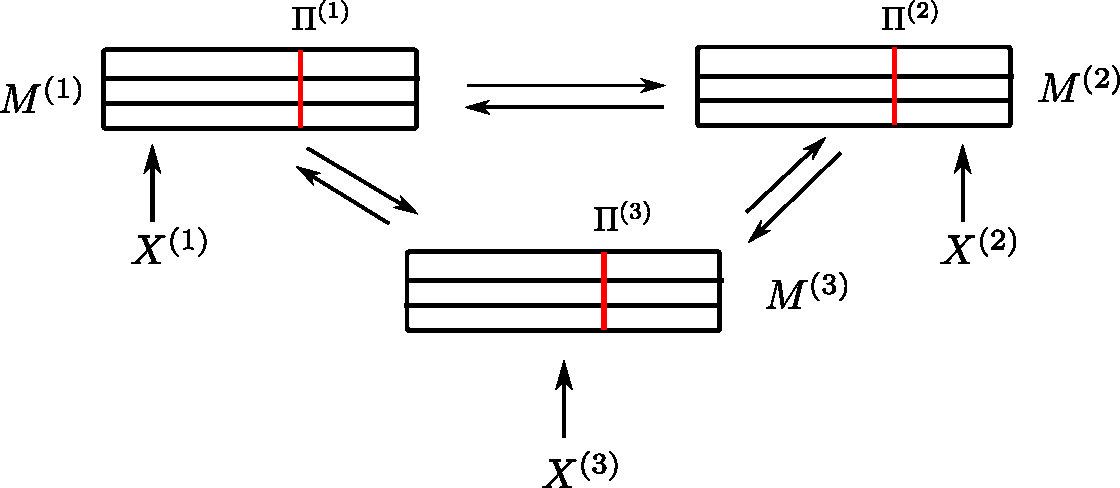
\includegraphics[width=0.6\textwidth]{archi_3maps.pdf}
	\vspace{-0.5cm}
	\caption{Architecture de trois cartes utilisée dans les expériences. Chaque carte prend une entrée externe $\inpx\m{i}$ et est connectée aux deux autres. Elle possède ainsi deux couches de poids contextuels et une couche de poids externes.\label{fig:archi_3maps}}
\end{figure}

\subsection{Méthode expérimentale}

Les tâches de prédiction de ce chapitre seront réalisées sur une architecture de trois cartes 1D, toutes connectées entre elles~; cette architecture est représentée en figure~\ref{fig:archi_3maps}.
Chacune des trois cartes prend une entrée externe en une dimension et deux entrées contextuelles qui sont les positions des BMUs des deux autres cartes. Elle possède donc deux couches contextuelles $\w_{c_0}$ et $\w_{c_1}$.
Nous construisons deux modèles d'entrées jouets à partir du cercle 2D et du patch $[0,1]^2$ en leur ajoutant une troisième dimension, de telle sorte à ce que la connaissance de deux entrées sur trois détermine la valeur de la troisième entrée. Pour cela, nous pivotons le plan 2D dans lequel se situent ces entrées dans un espace en trois dimensions.
Ces modèles, référencés par \textbf{G} et \textbf{H}, sont tracés en figure~\ref{fig:inputs_3D}.
Chaque carte de l'architecture prend en entrée une des coordonnées des points 3D du modèle.

\begin{figure}[h!]
	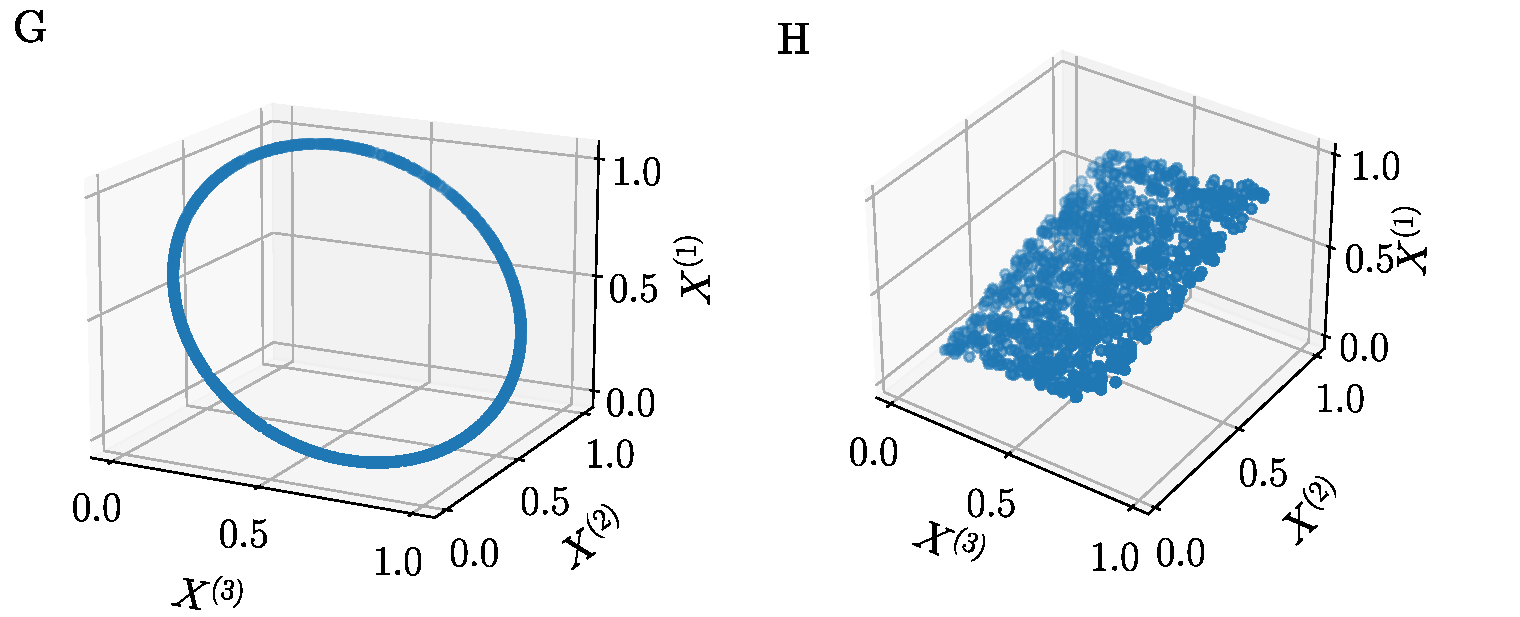
\includegraphics[width=\textwidth]{inputs/inputs_3D.pdf}
	\caption{Dispositions d'entrées en trois dimensions utilisées dans cette partie. Chaque carte $M\m{1}$, $M\m{2}$, $M\m{3}$ prend en entrée une coordonnée $\inpx\m{1}, \inpx\m{2}, \inpx\m{3}$. \label{fig:inputs_3D}}
\end{figure}

L'algorithme de prédiction d'entrée est schématisé en Figure~\ref{fig:schema_pred}.
La phase d'apprentissage du modèle est la même que dans les expériences précédentes~: les trois cartes reçoivent leurs entrées externes $\inpx\m{1},\inpx\m{2}, \inpx\m{3}$.
La phase de prédiction est une phase de test, durant laquelle les poids de toutes les cartes ne sont pas mis à jour.
Pour cette phase de prédiction, nous choisissons une carte, ici $M\m{1}$, comme carte prédictive. 
Cette carte ne reçoit plus son entrée externe, mais seulement ses entrées contextuelles. 
Les autres cartes reçoivent quant à elles leurs entrées externes $\inpx\m{2}$ et $\inpx\m{3}$.
La seule différence avec une phase de test classique est que la carte prédictive $M\m{1}$ prend comme activité globale sa seule activité contextuelle. Si la carte possède plusieurs couches de poids contextuels, il s'agit de la moyenne des activités contextuelles.
La valeur prédite récupérée en sortie de l'architecture est le poids externe du BMU de la carte prédictive $\w\ext\m{1}(\bmu\m{1})$.

Pour ces deux modèles d'entrées, nous vérifierons si les comportements d'organisation en zones de BMUs, observés sur deux cartes, sont également présents~; 
Nous effectuerons ensuite une phase de prédiction de l'entrée $\inpx\m{1}$ et vérifierons si la valeur prédite $\w\ext(\bmu\m{1})$ est proche de la valeur attendue $\inpx\m{1}$, qui n'a pas été présentée à la carte.

\begin{figure}
	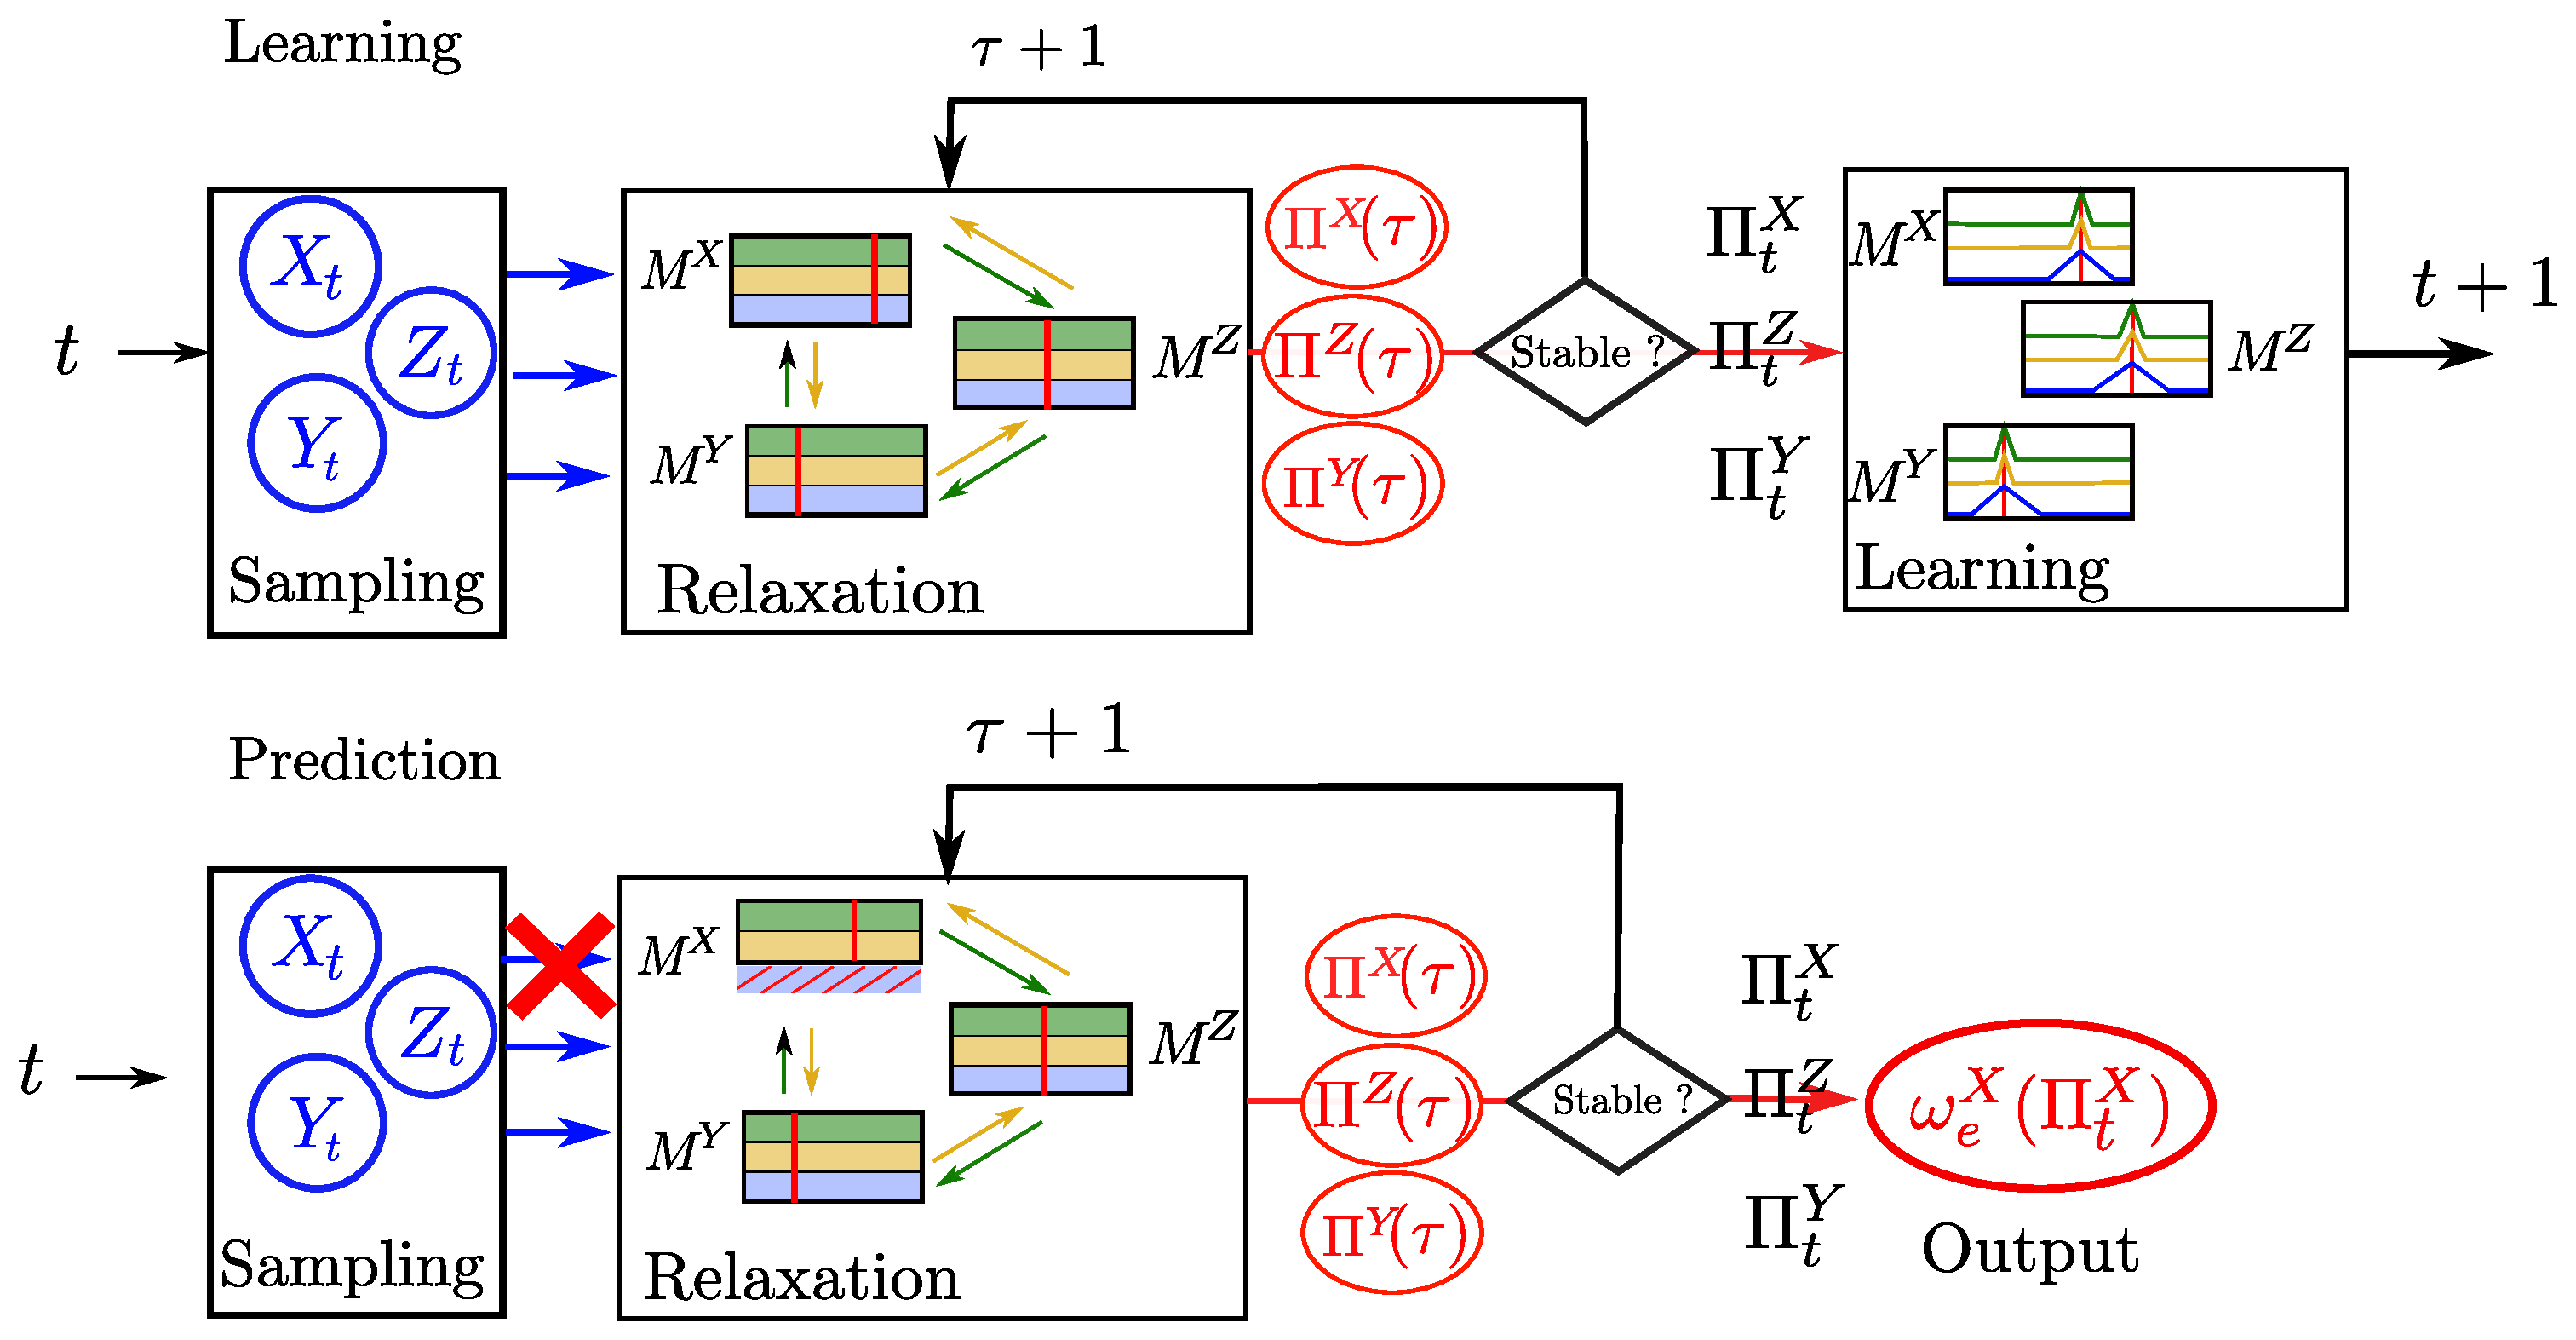
\includegraphics[width=\textwidth]{learning_tests.pdf}
	\caption{Schéma descriptif des opérations effectuées lors de l'apprentissage et de la phase de prédiction. Après une phase d'apprentissage classique, la phase de prédiction est une phase de test durant laquelle l'entrée $\inpx\m{1}$ n'est pas présentée à la carte $M\m{1}$. Celle-ci ne prend alors plus en compte son activité externe dans le calcul du BMU par relaxation. \label{fig:schema_pred}}
\end{figure}

\subsection{Résultats}

Nous traçons en figures \ref{fig:w_cercle} et \ref{fig:w_plan3} la représentation cartographique des trois cartes après apprentissage, dans les deux modèles d'entrées.
Nous observons d'abord que, comme pour deux cartes, les poids contextuels définissent un ensemble de zones dans lesquels tombent les BMUs.
Dans le cas du cercle \textbf{G}, toute valeur de $\inpx\m{1}$ peut correspondre à deux points différents du modèle d'entrées.
Les zones observées sur la représentation cartographique de $M\m{1}$ montrent que la carte choisit un BMU réagissant à $\inpx\m{1}$ de façon à différencier les deux valeurs possibles correspondantes dans le modèle d'entrée. 
Ce comportement étend ainsi celui observé sur deux cartes.
Ce même comportement est également observé pour le plan \textbf{H}.
Chaque carte a donc encodé le modèle d'entrée, et non seulement sa seule entrée externe.
Grâce à cet encodage, nous voulons maintenant observer si l'architecture est capable de prédire $\inpx\m{1}$ à partir des seules entrées $\inpx\m{2}$ et $\inpx\m{3}$.


\begin{figure}[h!]
	\centering\includegraphics[width=\textwidth]{cercle3D/weights.pdf}
	\caption{Représentation cartographique des poids et entrées dans l'architecture de trois cartes apprenant sur un cercle en trois dimensions. Nous observons la formation de zones similaires au cas en deux dimensions. \label{fig:w_cercle}}
\end{figure}

\begin{figure}[h!]
	\centering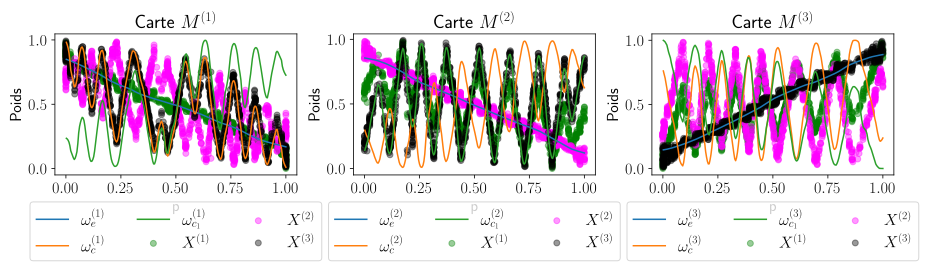
\includegraphics[width=\textwidth]{plan/weights_P2}
	\caption{Représentation cartographique des poids et entrées dans l'architecture de trois cartes apprenant sur un plan pivoté en 3D. Les zones sont similaires au cas en deux dimensions. \label{fig:w_plan3}}
\end{figure}


Nous traçons l'erreur obtenue lors de la phase de prédiction de $\inpx\m{1}$~: en figure \ref{fig:pred_cercle} pour le modèle du cercle \textbf{G}, et \ref{fig:plan3_pred} sur le plan \textbf{H}.
Dans les deux cas, l'entrée $\inpx\m{1}$ n'a pas été présentée à la carte et sa valeur est prédite par $\w\ext\m{1}(\bmu\m{1})$. 
Nous ajoutons aux tracés l'erreur de quantification vectorielle dans les autres cartes, qui ont reçu leur entrée externe, afin de comparer la qualité de la prédiction à la qualité de la quantification vectorielle.
Nous observons que la prédiction est très bien réalisée dans le cas du cercle. Les valeurs prédites par la carte $M\m{1}$ sont aussi précises que les valeurs quantifiées par les cartes $M\m{2}$ et $M\m{3}$.
L'architecture de cartes a donc encodé le modèle d'entrée et est capable de prédire l'entrée manquante.
Dans le cas du plan, la prédiction est également bien réalisée~: l'erreur sur la prédiction de l'entrée $\inpx\m{1}$ est équivalente à l'erreur réalisée par la quantification vectorielle dans les autres cartes.

\begin{figure}
	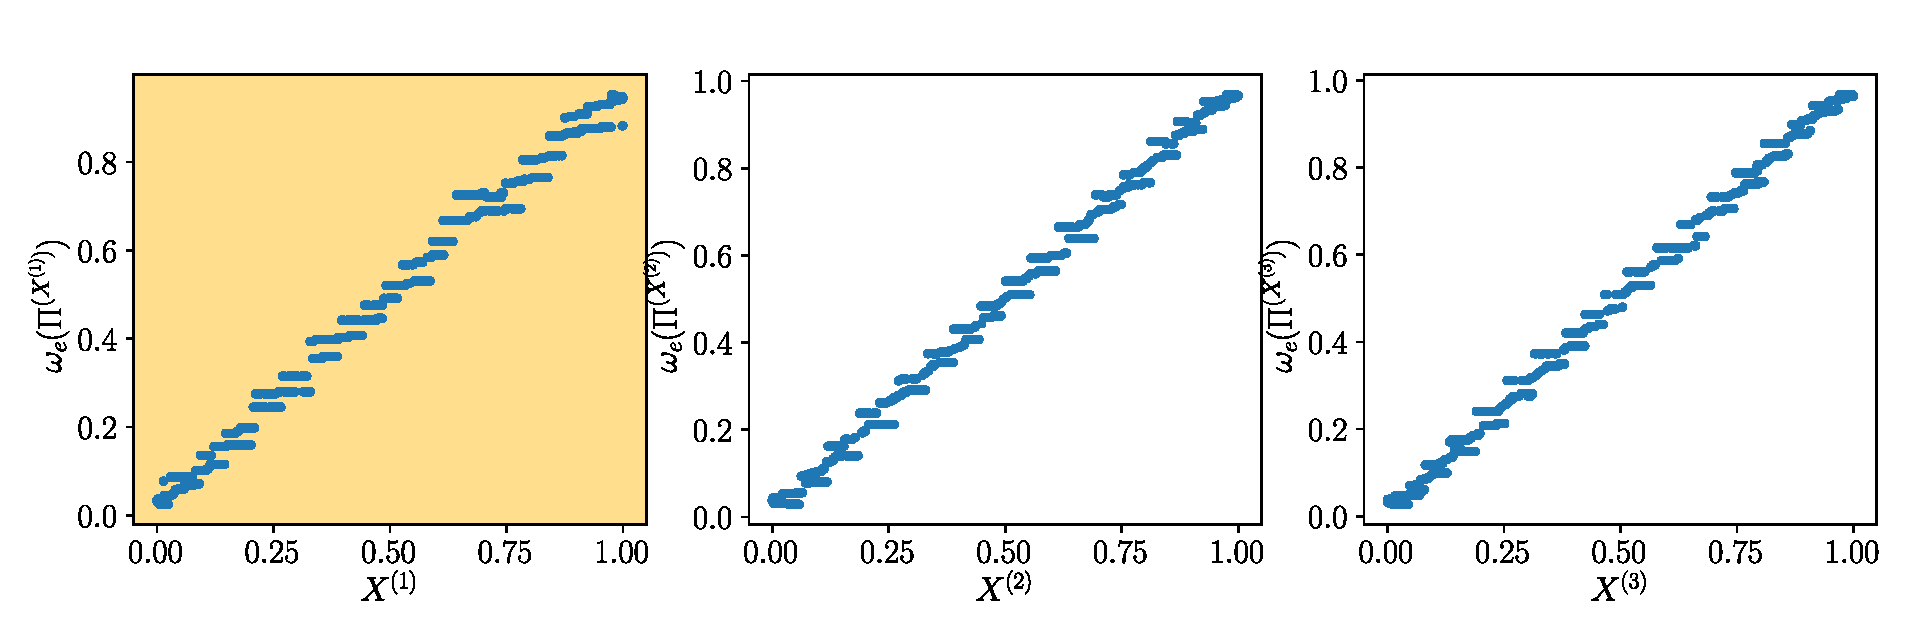
\includegraphics[width=0.95\textwidth]{cercle3D/error-closed-2.pdf}
	\caption{Erreur de prédiction de $\inpx\m{1}$ par $\w_e(\bmu\m{1})$ lorsque les entrées sont sur un cercle en trois dimensions. $\inpx\m{1}$ n'a pas été présenté à $M\m{1}$.
	 Les nuages de points correspondant à $M\m{2}$ et $M\m{3}$ correspondent à l'erreur de quantification dans les cartes 2 et 3 qui ont reçu leur entrée externe. Ces tracés montrent une bonne prédiction de $\inpx\m{1}$ par la carte 1. \label{fig:pred_cercle}}
\end{figure}

\begin{figure}
	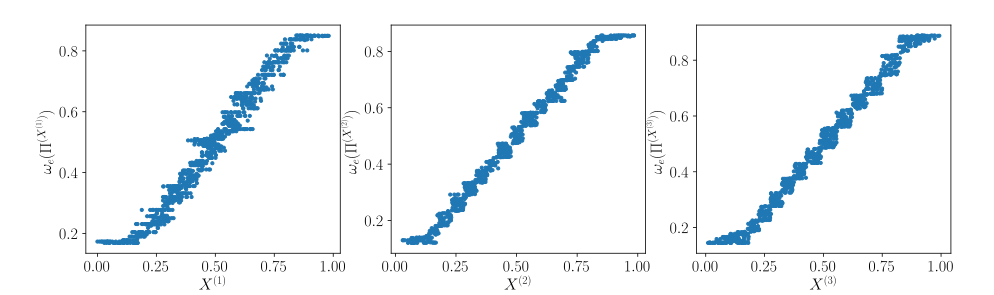
\includegraphics[width=\textwidth]{plan/zclosed-1-19999_error-P2}	
	\caption{Erreur de prédiction de $\inpx\m{1}$ dans le cas du plan pivoté en 3D. La prédiction effectuée par $M\m{1}$ est correcte. L'erreur est équivalente à la quantification vectorielle réalisée par $M\m{2}$ et $M\m{3}$. L'architecture de trois cartes est donc capable de prédire $\inpx\m{1}$. \label{fig:plan3_pred}}
\end{figure}

La disposition en étages qui apparaît sur les tracés d'erreur de prédiction se rapporte directement à la disposition en zones des cartes de l'architecture. Les entrées contextuelles reçues par $M\m{1}$ permettent à la carte de sélectionner une des zones définies par les poids contextuels.
Afin de valider l'importance de la disposition en zones dans la capacité de prédiction d'entrée, nous nous intéressons à la prédiction dans un cas ou les cartes ne se seraient pas organisés en zones.
Pour cela, nous effectuons une phase d'apprentissage et prédiction sur une architecture dans laquelle $r_c = r_e$. 
Nous avions vu que ce choix de paramètres n'engendre pas la formation de zones. L'erreur de prédiction qui en résulte est tracée en figure $\ref{fig:rcre_pred}$.
Nous observons que dans cette configuration, l'architecture de cartes n'est pas capable de réaliser la prédiction d'entrée manquante.
Bien que cette architecture ait appris sur les trois entrées du modèle, ne pouvons pas parler d'un apprentissage du modèle dans ce cas, car les cartes ne sont pas capables d'utiliser les relations entre entrées dans la tâche de prédiction.
Les zones permettent donc bien aux cartes d'encoder les relations entre entrées et de les réutiliser en sortie. Elles sont caractéristiques de l'apprentissage du modèle d'entrée par l'architecture.

\begin{figure}
	\centering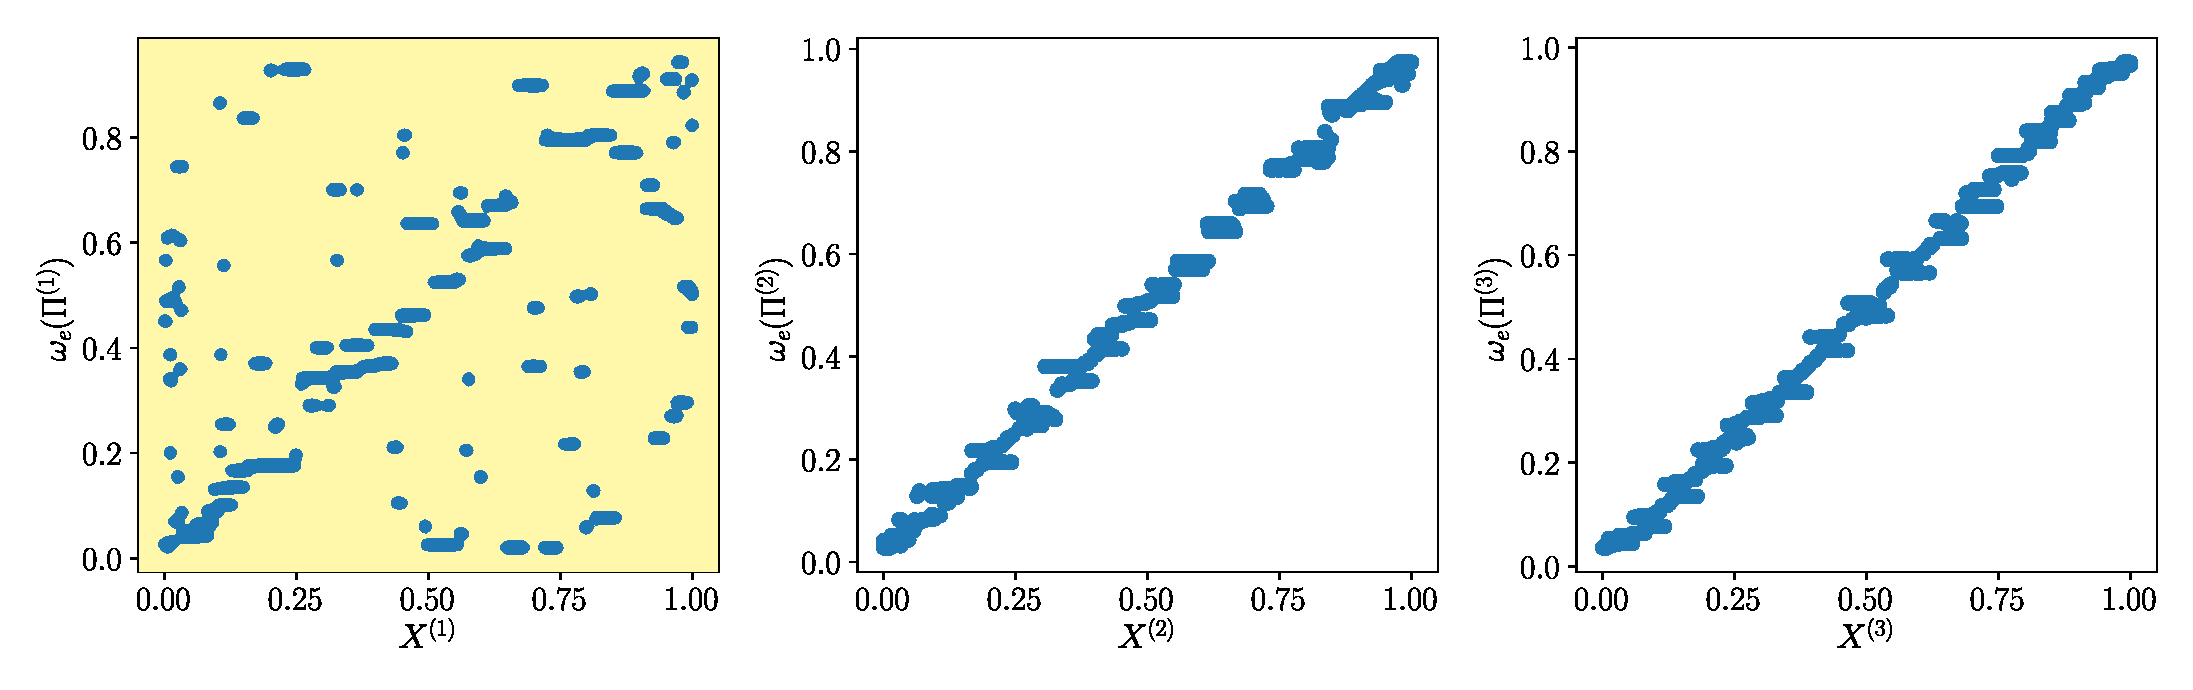
\includegraphics[width=0.9\textwidth]{rceqre/prediction.pdf}
	\caption{Prédiction de l'entrée $X\m{1}$ lorsque $r_c = r_e$. La prédiction n'est pas effectuée. Ainsi, sans formation de zones, la capacité de prise de décision n'est plus réalisable par une carte de l'architecture. \label{fig:rcre_pred}}
\end{figure}

\subsection{Conclusion}

Nous avons donc montré qu'une architecture de cartes est capable de générer une modalité manquante dans le modèle grâce aux connexions entre cartes. La valeur utilisée pour la prédiction est dans ce cas le poids externe du BMU de la carte qui n'a pas reçu son entrée externe.
Ce comportement montre que grâce aux poids appris et à la recherche de BMU, une architecture de cartes est non seulement capable d'encoder un modèle d'entrée, mais également de le réutiliser de façon autonome~: la génération d'entrée est réalisée par le même algorithme que celui utilisé lors des phases de tests.
Les connexions d'une architecture sont rétroactives, aussi n'importe quelle carte de l'architecture peut être utilisée comme carte prédictive, ce qui constitue un avantage d'une architecture non-hiérarchique.

Nous avons observé que les zones de poids contextuels permettent cette capacité de prédiction. Ce comportement est donc bien un marqueur de l'apprentissage du modèle par une architecture de cartes. Le fait que l'entrée générée corresponde directement à la valeur de l'entrée manquante vient de la quantification vectorielle sur l'entrée externe qui est effectuée au sein de chaque carte.

\section{Exemple d'application de la prédiction d'entrée au contrôle d'un drone en vol}

Nous avons observé qu'après apprentissage, une architecture de cartes est capable de générer une entrée manquante de façon autonome. Cette entrée est en adéquation avec le modèle d'entrées apprises par l'architecture~: il s'agit d'une prédiction.
Nous sortons du cadre des entrées simulées pour nous placer dans un cas de contrôle réel. 
Cette expérience est un exemple simple d'application de l'architecture en robotique, qui nous permet de tester les cartes sur des entrées bruitées, dont nous ne connaissons pas le modèle de relation.

Nous disposons d'un drone contrôlé à distance par ordinateur. 
Ce drone possède une caméra frontale ainsi qu'un ensemble de capteurs internes. Chacun des capteurs du drone est une modalité d'un espace multimodal. Leurs valeurs dépendent les unes des autres~: elles dépendent par exemple de la position du drone à un instant.
La commande envoyée au drone à chaque instant peut également être considérée une modalité de l'environnement. 
Lorsque le drone cherche à suivre une trajectoire donnée, la commande envoyée à chaque instant devient dépendante des valeurs des capteurs.

\`A l'aide d'une architecture de cartes, nous voulons ainsi apprendre les relations existant entre les capteurs et la commande, afin de pouvoir générer la commande à envoyer au drone à partir des valeurs des capteurs lors d'une phase de prédiction.
Nous effectuerons cette phase de prédiction en temps réel, pendant laquelle la commande prédite sera envoyée au drone à chaque instant.
Le but de cette expérience est de tester l'architecture de cartes sur des cas d'entrées réelles, donc bruitées, en se plaçant dans un cadre de contrôle en temps réel d'un drone.
Nous évaluerons la robustesse de l'algorithme à des données bruitées et la capacité de CxSOM à réagir en temps réel malgré les étapes de relaxation.

\subsection{Méthode expérimentale}

Le drone utilisé pour l'expérience est un quadricoptère. Il possède une caméra frontale non orientable.
Nous le contrôlons à distance par un ordinateur.  Lors de cette expérience, le drone naviguera dans un couloir en ligne droite. L'objectif du contrôle est que le drone se déplace au centre du couloir, en ligne droite.


La figure \ref{fig:drone} présente les capteurs et commandes disponibles.
Le drone est commandé par la définition d'un angle de rotation autour de chaque axe. 
L'angle autour de l'axe $z$, noté $\w$, contrôle la vitesse de rotation angulaire du drone autour de cet axe (lacet).
L'angle autour de l'axe $y$ (tangage) contrôle la vitesse de rotation haut/bas. Enfin, l'angle autour de $x$, que nous notons $\rho$ (roulis), influence l'\emph{accélération} du drone selon $y$. Dans cette expérience, nous contrôlerons uniquement l'angle de roulis $\rho$ à l'aide de l'architecture de cartes.
L'angle de lacet $\omega$ sera contrôlé à l'aide d'un PID de façon à ce que la caméra du drone reste dirigée vers le milieu du couloir. L'angle de tangage $y$ est maintenu à 0 à l'aide d'un PID, de façon à ce que le drone se déplace à une altitude constante.
La commande $\rho$ constitue une première modalité des entrées que nous allons considérer pour l'apprentissage de l'architecture de cartes.

Nous considérons trois éléments extraits des capteurs du drone et qui sont relatifs à sa position par rapport au couloir. Une analyse de l'image issue de la caméra frontale nous permet de récupérer l'abscisse du point de fuite du couloir $x$ et la différence entre les angles des lignes du couloir, notée $\varphi$.
Enfin, les capteurs internes du drone nous permettent de récupérer les vitesses linéaires $v_x,v_y,v_z$ à chaque instant selon chaque axe de déplacement. 
Comme nous contrôlerons l'angle $\rho$, donc une l'accélération linéaire selon $y$, nous nous intéresserons particulièrement à la vitesse linéaire en $y$ en tant que modalité.
Finalement, nous utiliserons quatre modalités lors du déplacement du drone~: l'abscisse du point de fuite $x$, l'angle duy couloir $\varphi$, la commande en angle de roulis $\rho$ et la vitesse linéaire courante en $y$ $v_y$.


Nous construisons une architecture CxSOM sur ces quatre modalités, composée de quatre cartes 1D connectées chacune aux trois autres, tracée en figure~\ref{fig:archi_drone}. Chaque carte prend une des modalités comme entrée externe.
Le but de l'architecture sera de capturer les relations entre les capteurs et la commande puis générer la commande lors de la phase de prédiction.
La phase d'apprentissage est réalisée sur des trajectoires du drone dans le couloir lorsque la commande est réalisée par un humain.
Lors de cette phase, nous avons utilisé un système de contrôle PID pour assister la commande humaine. 
Cette phase d'apprentissage est réalisée hors ligne~: nous normalisons d'abord les entrées puis les présentons aléatoirement lors de la phase d'apprentissage.
Chaque carte est de taille $500$. Les paramètres sont $r_e = 0.2$ et $r_c = 0.02$.
L'apprentissage a été effectué sur 4890 points, obtenus sur des trajectoires effectuées dans le même couloir que les trajectoires de test. Nous avons présenté ces points une seule fois, ce qui a suffi à un bon dépliement des cartes.


Après apprentissage, nous effectuons une phase de prédiction en ligne et en temps réel sur le contrôle du drone.
Lors de cette étape, la commande $\rho$ n'est pas présentée à la carte $M\m{\rho}$. $\w_e\m{\rho}(\bmu\m{\rho})$ et la valeur de la prédiction est utilisé comme commande $\rho$ envoyée au drône en temps réel.
Les angles de tangage et de lacet sont quant à eux contrôlés par un PID afin de maintenir l'axe du drone pointant vers le centre du couloir et une altitude constante.

\begin{figure}
	\centering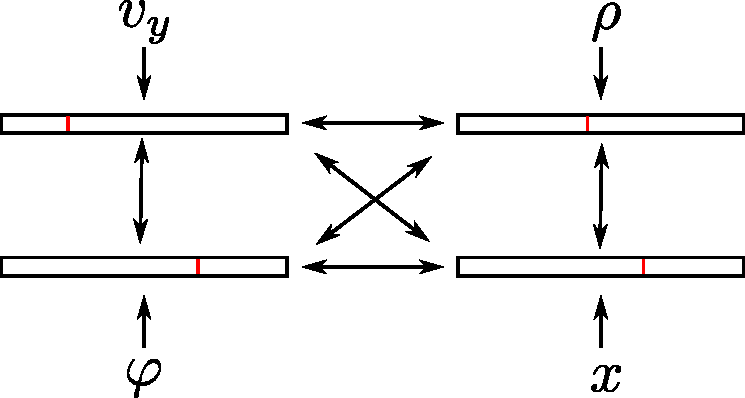
\includegraphics[width=0.5\textwidth]{archi_drone.pdf}
	\caption{Architecture de quatre cartes utilisée dans l'expérience. Chaque carte prend une modalité en entrée externe lors de l'apprentissage~: $v_y,\rho,\varphi,x$. Lors de la phase de prédiction, l'entrée $\rho$ n'est plus présentée à l'architecture et la commande envoyée au drône est $\w_e\m{\rho}(\bmu\m{\rho})$\label{fig:archi_drone}}.
\end{figure}

Afin de mieux visualiser les conditions de l'expérience, nous avons tracé les dépendances entre chaque modalité en figure~\ref{fig:drone_inp}.
Nous nous intéressons ici aux dépendances entre la commande $\rho$ qui est celle que nous prédirons et des autres modalités.
On remarque que $\rho$ dépend linéairement de l'angle du couloir $\varphi$, mais que cette dépendance est très bruitée. Elle dépend également de la vitesse interne du drone $v_y$. Par contre, les entrées correspondant à l'abscisse du point de fuite varient peu~; la commande $\rho$ dépend peu de $x$.

\begin{figure}
	\begin{minipage}{0.5\textwidth}
	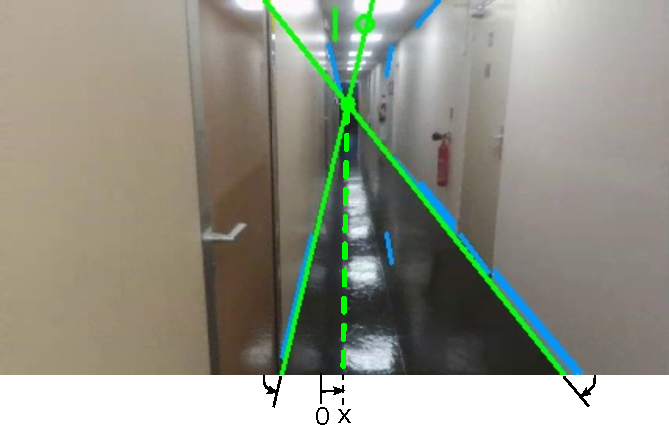
\includegraphics[width=\textwidth]{visudrone.pdf}
	\end{minipage}
	\begin{minipage}{0.5\textwidth}
	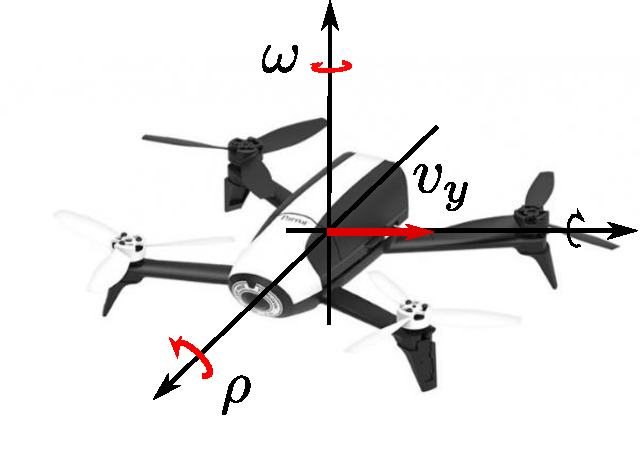
\includegraphics[width=\textwidth]{dronesteup}
	\end{minipage}
	\caption{Disposition des capteurs utilisés pour l'expérience}
	\label{fig:drone}
	\end{figure}

\begin{figure}
	\centering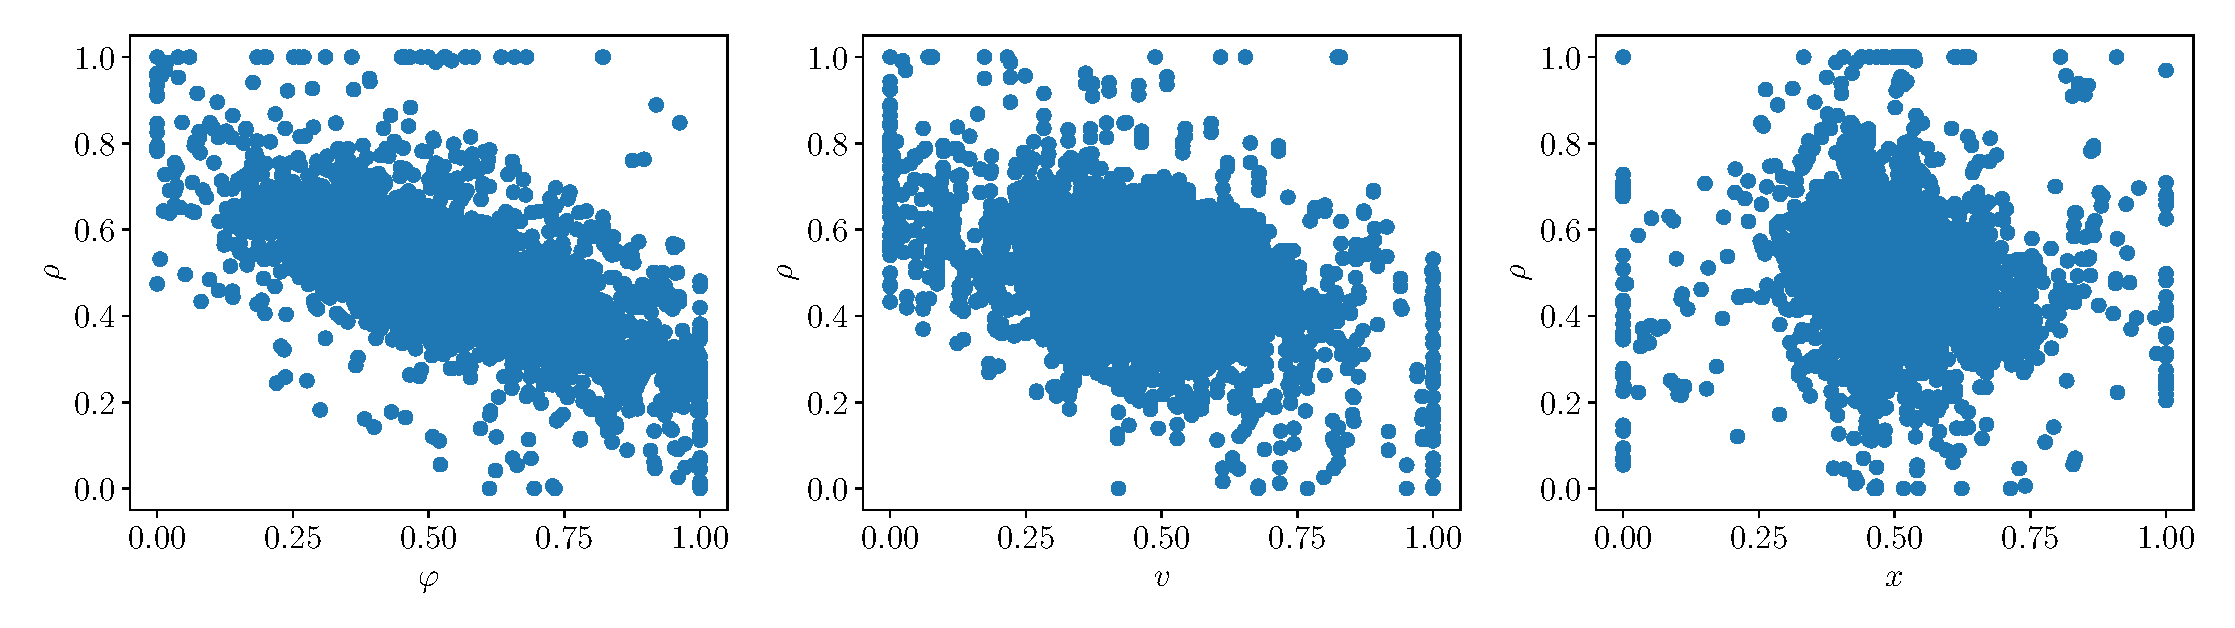
\includegraphics[width=\textwidth]{drone_inputs}
	\caption{Disposition et dépendances des entrées d'apprentissage. Nous chercherons à prédire $\rho$~: cette valeur dépend bien des autres modalités $v$, $\varphi$ et $x$. La dépendance est très simple (linéaire) mais très bruitée, et $\rho$ ne dépend pas de $x$. \label{fig:drone_inp}}
\end{figure}


\subsection{Résultats}

La carte associée à $\rho$ possède une couche de poids externe et trois couches de poids contextuels. 
Ces poids sont représentés en figure \ref{fig:drone_w}. 
Nous observons d'abord que l'organisation des poids contextuels rappelle celle observée dans les dispositions d'entrées jouets~: les poids contextuels définissent des zones. 
La figure~\ref{fig:drone_w} présente en violet un exemple de calcul d'activité de la carte $\rho$ pendant la phase de prédiction.
A un instant $t$, l'architecture reçoit les trois modalités $v_y, x, \varphi$.
L'activité de $M\m{\rho}$ représentée est son activité contextuelle globale après la relaxation, calculée seulement grâce à ses entrées contextuelles.
Le BMU correspond au maximum de l'activité~: $\bmu\m{\rho} = 0.41$ et la valeur de prédiction est $\w_e(\bmu\m{\rho}) = 0.49$. Cette valeur, remise à l'échelle, est la commande que nous envoyons au drone à l'instant $t$.
Tous ces calculs doivent être réalisés assez rapidement pour que le drone réagisse en temps réel.

Lors des expériences que nous avons effectuées, le drone apparaît voler correctement dans le couloir sans toucher les murs. Nous observons cependant que cette trajectoire est assez imprécise~: la commande prédite permet au drone de ne pas toucher les murs, mais ne lui permet pas de se centrer finement au centre du couloir.
La prédiction est donc correctement réalisée, toutefois assez imprécise. 
Le fait que les entrées soient très bruitées peut expliquer ce manque de précision. 
% Par ailleurs, ce type de contrôle manque de rétroaction, même en utilisant $v_y$ dans le calcul de la commande, d'où l'instabilité sur la trajectoire.

\subsection{Conclusion}

Cette application sur une architecture de quatre carte nous permet d'abord d'étendre les observations réalisées sur deux et trois cartes et montre que les comportements des architectures de deux et trois cartes, à savoir la formation de zones, sont également observés sur les 4 cartes.
Ensuite, la capacité de prédiction observée sur le drone constitue une possibilité conceptuelle d'application des architectures de cartes sur des données réelles. 
Malgré les données bruitées, l'architecture de cartes détecte une relation entre entrées qui lui permet de prédire de façon large la commande à envoyer.
Enfin, la réactivité de l'envoi de la commande au drone montre que la relaxation permet quand même une réponse en temps réel.


Ces observations sont sur un cas simple d'application en une dimension, mais laissent la porte ouverte à une application possible des architectures CxSOM en pratique, par exemple en robotique. 
Nous pouvons imaginer, à plus grande échelle, que l'architecture de carte permette à un robot une prise de décision par rapport à la disposition de ses capteurs. La capacité de prédiction laisse également envisager des applications de robustesse à un capteur cassé ou l'utilisation de données dans lesquelles il manque parfois une modalité.
Une réelle application de l'architecture peut donc être une piste d'étude future.
Dans ce sens, il serait intéressant d'étudier l'application sur des données moins bruitées et disponibles en simulation afin de mesurer l'erreur de prédiction relative à l'architecture, comme une étape intermédiaire entre les données géométriques et le cadre réel. 
L'architecture de carte pourra être combinée à d'autres modèles de contrôle automatique pour stabiliser les commandes envoyée au robot.
Enfin, les entrées d'une application en robotique sont en pratique en plus grande dimension~: ce sont par exemple directement des images. Il sera nécessaire d'étudier l'organisation des cartes sur des données en grande dimension pour envisager une application, en utilisant dans ce cadre des cartes en deux dimensions.

\begin{figure}
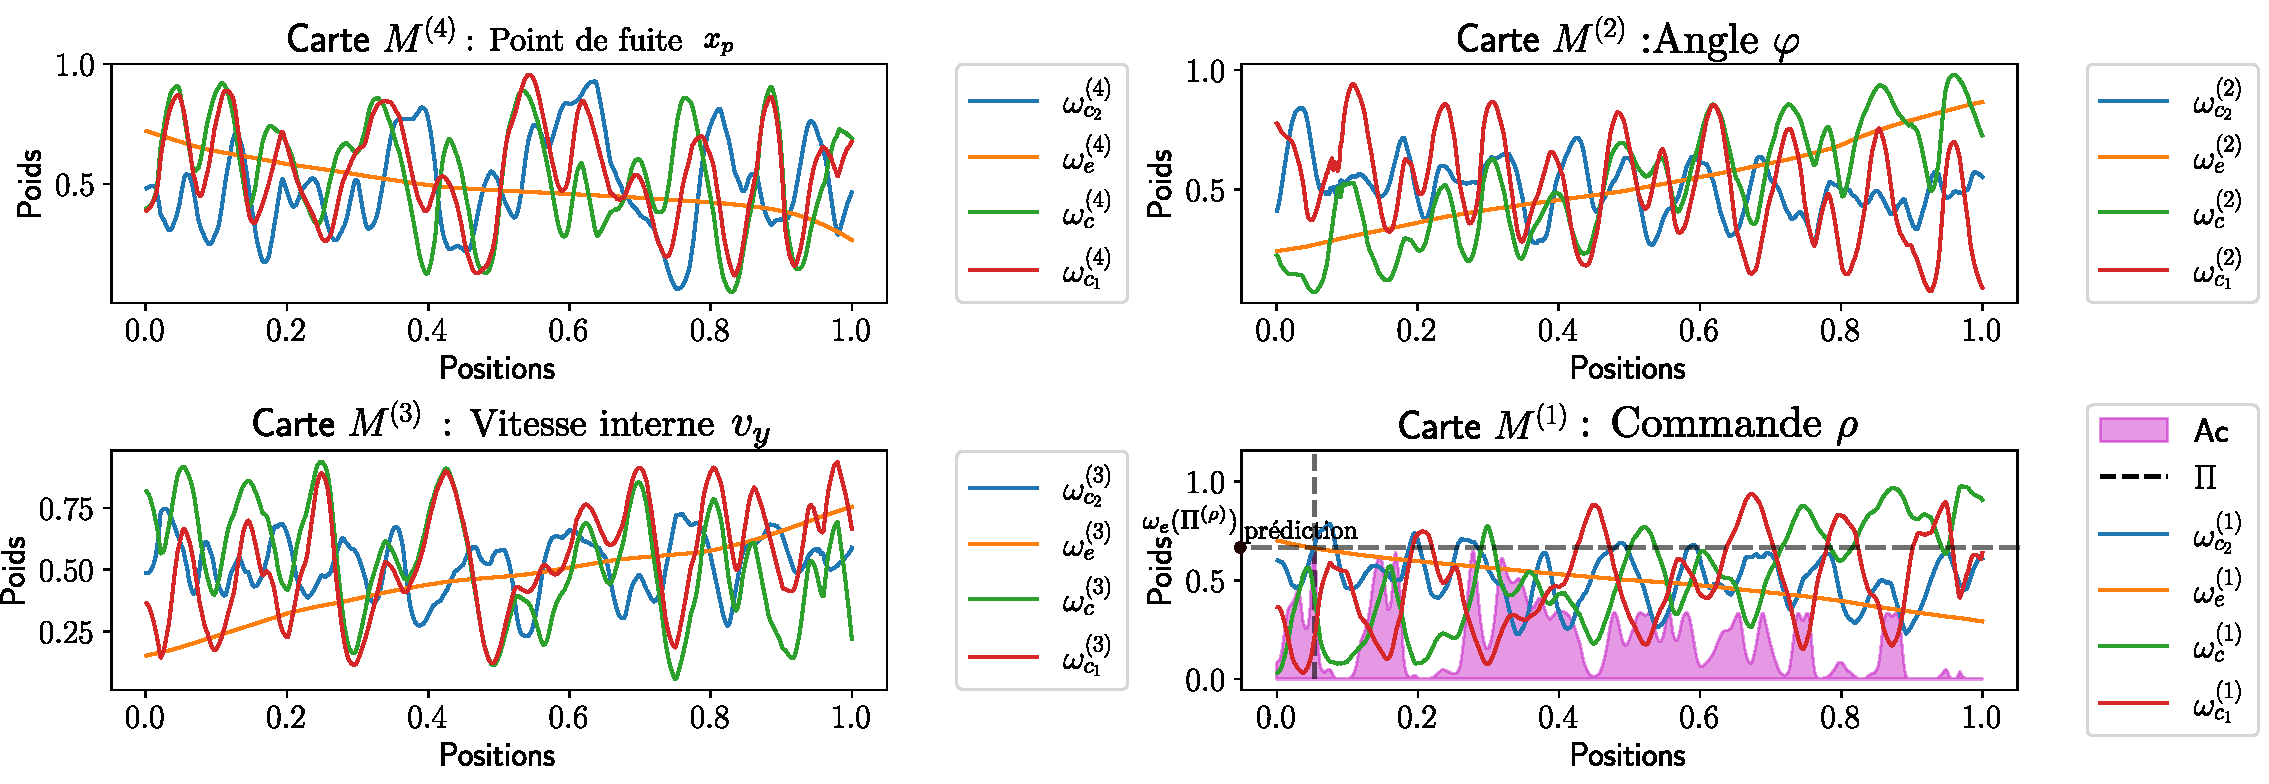
\includegraphics[width=\textwidth]{drone_weights.pdf}
\caption{Disposition des poids des 4 cartes après apprentissage. La commande prédite $\rho$ envoyée au drone est le poids externe du BMU de la carte $\rho$, calculé uniquement à partir des activités contextuelles. Cette activité est représentée en violet sur la dernière carte.}
\label{fig:drone_w}
\end{figure}

\section{Influence des connexions d'une architecture sur l'apprentissage du modèle d'entrée}

Dans toutes les expériences précédentes, nous avons utilisé des architectures dans lesquelles les cartes sont toutes connectées. Or, le nombre d'architectures de cartes différentes possibles augmente ensuite exponentiellement avec le nombre de cartes considérées pour une architecture.
L'influence des connexions sur l'apprentissage d'un modèle d'entrée est donc une orientation judicieuse pour nos futurs travaux sur CxSOM. 
Nous présentons dans cette dernière partie deux observations ouvrant des questions sur l'influence des connexions dans une architecture.
Nous étudierons d'abord un exemple d'architecture dans laquelle chaque carte possède un grand nombre de connexions.
Nous nous intéresserons ensuite à l'influence qu'ont sur une carte de l'architecture les cartes qui ne lui sont pas directement connectées.

\subsection{Influence d'un grand nombre d'entrées contextuelles sur l'organisation d'une carte}

Nous avons vu qu'une architecture de deux cartes apprenant sur le patch $[0,1]^2$ se déplie de manière à former deux échelles d'indices. 
Nous voulons étendre cette expérience pour des entrées de plus grande dimension et une architecture de plus de cartes. 
Nous choisissons d'effectuer une expérience dans laquelle toutes les modalités sont indépendantes, mais cette fois pour 9 cartes toutes connectées.
Nous tirons donc les entrées des cartes dans l'hypercube $[0,1]^9$. 
Nous ajoutons à ces $9$ entrées indépendantes une entrée $\inpx\m{10}$ identique à l'entrée $\inpx\m{9}$ pour construire finalement une architecture de 10 cartes, toutes connectées. Chaque carte possède une couche externe et 9 couches contextuelles.
Nous voulons observer deux comportements~: 
\begin{itemize}
	\item Comment la présence de nombreuses entrées contextuelles modifient le choix du BMU, par rapport à la présence d'une seule entrée contextuelle ? 
	\item La relation entre les entrées $\inpx\m{9}$ et $\inpx\m{10}$ est-elle encodée au sein des cartes, ou cette relation est cachée par toutes les connexions relatives à des entrées indépendantes ? 
\end{itemize}

La figure \ref{fig:bigdim} présente la forme des poids de quatre des cartes dans l'architecture de 10 cartes~: les cartes $M\m{9}$ et $M\m{10}$, dont les entrées externes sont identiques, et les cartes $M\m{1}$ et $M\m{2}$, dont les entrées sont indépendantes de toutes les autres entrées.
Dans chacune des cartes, nous pouvons noter que les poids contextuels qui correspondent à des connexions entre cartes dont les entrées sont indépendantes se rapprochent tous d'une valeur moyenne constante de 0.5 dans chaque carte. \`A la fin de l'apprentissage, les activités contextuelles correspondant à ces couches de poids seront constantes sur toute la carte et n'interviennent alors plus dans le choix du BMU.
L'architecture équivaut donc à 9 cartes indépendantes, ce qui est cohérent par rapport à la disposition des entrées. 
Les couches de poids contextuels correspondant aux deux cartes dont les entrées sont identiques $\inpx\m{9}$ et $\inpx\m{10}$ sont représentées en rose dans $M\m{9}$ et $M\m{10}$. 
Elles se déplient totalement, comme nous l'avions observé en figure~\ref{fig:id_results}. Cette couche de poids sera ainsi la seule à réellement intervenir dans le choix du BMU et l'architecture a encodé cette relation.
En bas de la figure, nous traçons également observer la prédiction de l'entrée $\inpx\m{9}$. 
Elle est correctement réalisée lorsque la carte $M\m{9}$ ne reçoit pas son entrée externe. Les connexions \og inutiles \fg{} perturbent donc peu l'apprentissage des relations entre entrées. 
Finalement, les cartes $M\m{9}$ et $M\m{10}$ ont appris à effacer du calcul de l'activité les entrées indépendantes de leur entrée externe, et gardé les entrées contextuelles qui ont une relation avec leur entrée externe.

Cette expérience propose une idée de comportement à grande échelle à explorer plus en détail.
En particulier, on peut se demander si ce comportement peut permettre d'extraire automatiquement des relations entre entrées. Cette détection de relations serait un comportement émergent d'une architecture de cartes.

\begin{figure}
	\begin{minipage}{\textwidth}
	\includegraphics[width=\textwidth]{bigdim/weights.pdf}
	\end{minipage}
\begin{minipage}{\textwidth}
	\centering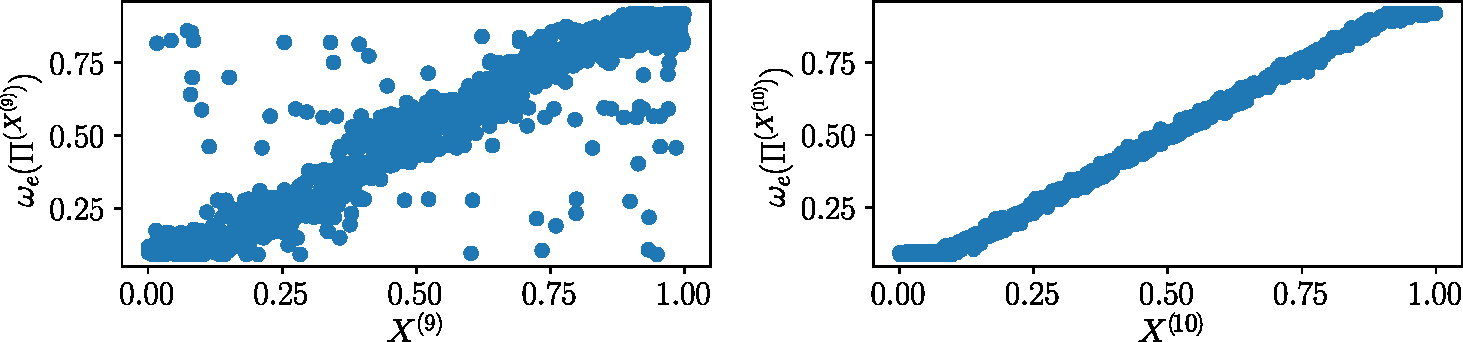
\includegraphics[width=0.8\textwidth]{bigdim/error_closed.pdf}
	\caption{En haut, tracé des poids des cartes pour une architecture de 10 cartes toutes connectées. Nous avons ici seulement tracé 4 cartes sur les 10. Les entrées sont toutes indépendantes, sauf les entrées $\inpx\m{9}$ et $\inpx\m{10}$ qui sont identiques. Nous remarquons que les poids contextuels se moyennent autour de 0.5, sauf ceux correspondant aux entrées dépendantes. En bas, nous traçons l'erreur de prédiction de la carte 9 lorsqu'elle ne reçoit pas d'entrée. La prédiction est bien réalisée~: les connexions contextuelles inutiles ne perturbent pas l'apprentissage. \label{fig:bigdim}}
\end{minipage}
\end{figure}

\subsection{Influence des connexions distantes sur l'organisation d'une carte}

Nous cherchons maintenant à observer comment une carte d'une architecture peut influencer une carte qui ne lui est pas directement connectée.
Dans cette deuxième expérience, nous repassons sur une architecture de trois cartes 1D et reprenons comme modèle entrée le cercle en trois dimensions (\textbf{G)}. 
Nous comparons le comportement d'une architecture dans laquelle les cartes sont connectées réciproquement, présentée plus haut, à celui d'une architecture de trois cartes connectées en boucle, dans laquelle chaque carte est uniquement connectée à une seule autre carte. 
Ce modèle d'architecture est illustré en figure~\ref{fig:archi_loop}~: $M\m{1}$ est connectée à $M\m{2}$, $M\m{2}$ connectée à $M\m{3}$ et $M\m{3}$ connectée à $M\m{1}$.

En particulier, nous observerons si l'architecture en boucle est capable de prédire $\inpx\m{1}$. 
Dans ce cas, la carte prédictive $M\m{1}$ ne reçoit en entrée que la position du BMU de $M\m{3}$~: la position du BMU de $M\m{2}$ intervient seulement de façon distante dans le calcul de l'activité de $M\m{1}$.
Afin de dissocier l'influence de $M\m{2}$ et $M\m{3}$ dans la prédiction de $\inpx\m{1}$, nous réalisons également une phase de prédiction effectuée uniquement à partir des cartes $M\m{3}$ et $M\m{1}$, sur les mêmes entrées et les mêmes dispositions de poids que dans l'architecture en boucle.
Dans le premier cas, $M\m{2}$ contribue à la prédiction via $M\m{3}$.
Elle n'intervient pas dans le second cas.

\begin{figure}[h!]
	\centering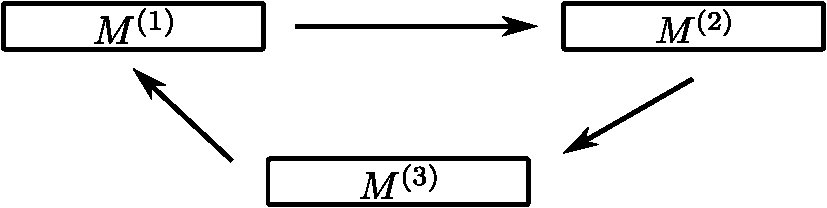
\includegraphics[width=0.5\textwidth]{loop/archi.pdf}
	\caption{Schéma de connexions d'une architecture en \og boucle\fg{}. \label{fig:archi_loop}}
\end{figure}

La disposition des poids est tracée en figure~\ref{fig:3som_loop}.
Les poids des cartes montrent une organisation similaire au cas où les connexions sont réciproques~: les poids contextuels forment des zones et chaque carte différencie ses BMUs en fonction du modèle d'entrée $U$ et non seulement de son entrée externe.
D'après la méthode d'étude présentée plus haut, nous pourrions dire que l'architecture a encodé le modèle d'entrées.

En figure~\ref{fig:pred_loop}, nous représentons la valeur de la prédiction dans l'architecture de trois cartes en fonction de l'entrée théorique $\inpx\m{1}$. Nous comparons cette prédiction à une prédiction effectuée uniquement grâce à $M\m{3}$.
Nous remarquons d'abord que la prédiction est moins bien réalisée dans l'architecture en boucle que dans l'architecture avec rétroaction~: les valeurs prédites ayant une erreur de moins de 0.1 par rapport à leur entrée théorique, marquées par les points rouges, représentent seulement 55 \% des 2000 entrées présentées lors du test.
L'architecture en boucle n'a donc pas aussi bien appris le modèle d'entrée que dans le cas où les trois cartes sont connectées réciproquement, dans laquelle plus de 99 \% des valeurs sont prédites avec une erreur de moins de 0.1 (cf. figure~\ref{fig:3som_pred}).
Cependant, la prédiction est mieux réalisée dans l'architecture en boucle à partir de $\inpx\m{3}$ et $\inpx\m{2}$ à distance, que lorsqu'on ne prend en compte que la valeur de $\inpx\m{3}$ pour la prédiction. 
Dans ce dernier cas, seules 40\% des entrées ont été correctement prédites par le couple de cartes~; l'erreur est globalement plus importante.
Cela montre que $M\m{2}$ intervient dans la prédiction de $\inpx\m{1}$, dans une faible mesure.

Cette observation montre qu'une carte conserve une influence à distance dans une architecture. 
Par contre, cette influence est minime par rapport à l'influence d'une connexion directe.
L'influence de ces connexions distantes est ainsi une piste d'étude pour un passage sur une grande architecture, dans laquelle nous pourrons agir sur les connexions entre cartes.

\begin{figure}[h!]
		\centering\includegraphics[width=\textwidth]{loop/weights_001.pdf}
		\caption{Poids à l'issue de l'apprentissage dans une architecture de 3 cartes connectées en boucle. Les poids contextuels forment des zones de BMUs similaires à celles observées dans l'architecture avec des connexions réciproques.\label{fig:3som_loop}}
\end{figure}

\begin{figure}[h!]
	\centering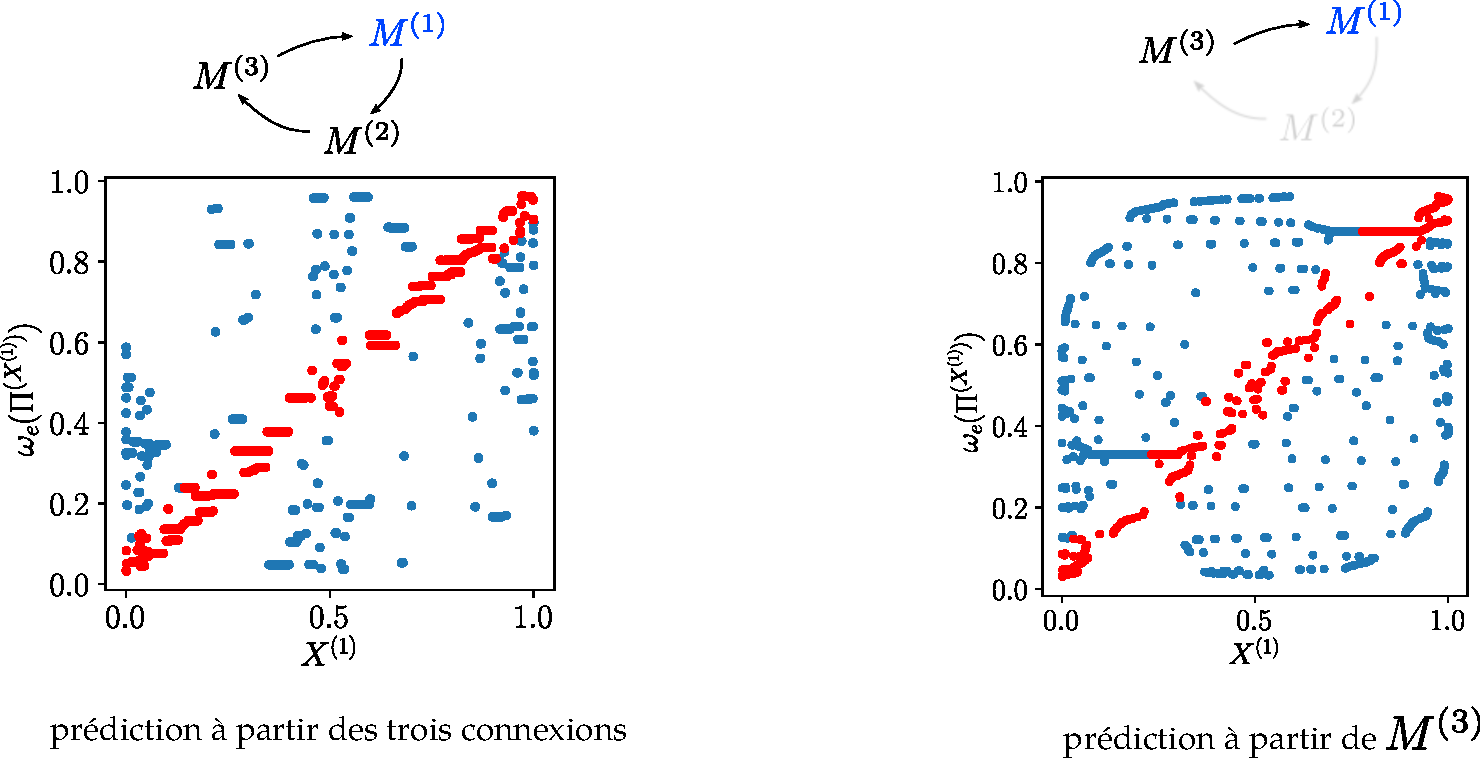
\includegraphics[width=0.9\textwidth]{loop/prediction_comparaison.pdf}
	\caption{\`A gauche, erreur de prédiction de l'entrée $\inpx\m{1}$ par l'architecture en boucle. Les points marqués en rouge représente les valeurs correctement prédites à moins de $0.1$ près. 
	\`A droite, nous représentons l'erreur de prédiction réalisée à partir des mêmes poids de cartes en ne prenant en compte que $M\m{1}$ et $M\m{3}$. La prédiction est moins bien réalisée que dans le cas de gauche, ce qui montre que $M\m{2}$ a bien une influence sur le calcul du BMU de $M\m{1}$ via $M\m{2}$.
	\label{fig:pred_loop}}
\end{figure}

\section{Conclusion}

Ce chapitre de résultats présente l'analyse de l'organisation d'architectures de 2 et 3 cartes 1D sur des données d'entrées en deux et trois dimensions.
Nous avons d'abord observé que l'apprentissage du modèle d'entrée dans une architecture CxSOM est marqué par une organisation à deux échelles~: les poids externes se déplient sur l'espace d'entrée comme les poids d'une carte classique. Les poids contextuels se déplient sur des sous-régions de la carte définies par la valeur de l'entrée externe, formant une disposition en \og zones \fg{}.
Ces zones de poids contextuels permettent d'encoder l'information sur tout le modèle d'entrée dans chacune des cartes~: 
chaque carte choisit son BMU en fonction à la fois de son entrée externe et de ses entrées contextuelles. Une position de BMU encode donc en une seule valeur $\bmu$ l'ensemble du modèle d'entrée et non seulement l'entrée externe de la carte.
Ces zones sont caractéristiques de l'apprentissage du modèle d'entrée par une architecture de cartes et sont observées sur de plusieurs jeux de données d'entrées jouets ou réelles, sur des architectures de deux et trois cartes, et quel que soit le nombre de connexions.

Nous avons ensuite constaté que l'organisation en zones permet à l'architecture d'utiliser le modèle appris pour générer des valeurs d'entrées manquantes.
Après apprentissage, une carte qui ne reçoit plus son entrée externe peut définir un BMU grâce à ses activités contextuelles.
Le poids externe du BMU peut être utilisé comme une valeur générée de la modalité qui n'a pas été présentée.
Dans ces tâches de prédiction, l'architecture CxSOM utilise le fait qu'elle ait encodé le modèle d'entrée. Une prédiction peut-être réalisée par n'importe quelle carte grâce aux connexions non-hiérarchique, et s'appuie sur le même algorithme que celui utilisé lors des tests.
Nous avons observé que la capacité de prédiction est directement liée à la présence des zones de poids contextuels, ce qui valide le fait que l'encodage du modèle vient bien de cette organisation en zones.
Cette capacité de prédiction est une application possible des architectures de cartes et permet également d'évaluer l'apprentissage d'un modèle d'entrée par l'architecture lorsque ce modèle n'est pas connu en théorie.
% Ligne sur des perspectives de la capacité de prédiction


Maintenant que nous avons observé les comportements d'apprentissage dans des architectures de 2 et 3 cartes, une perspective principale d'étude de CxSOM est la construction d'architectures comportant plus de cartes.
Dans ces architectures, le choix des connexions entre cartes constitue un degré de liberté supplémentaire.
Pour mener à bien cette construction, une étude plus générale de l'influence des connexions permettra d'ajouter cette dimension à la conception de systèmes CxSOM.
Nous avons présenté dans ce chapitre deux perspectives d'influence des connexions entre les cartes.
D'une part, nous avons vu que des connexions distantes permettent toujours à l'architecture de cartes d'apprendre un modèle d'entrée. Cependant, lors de la prédiction, les cartes distantes de la carte prédictive ont moins d'influence que les cartes qui lui sont directement connectées. Cette observation montre que la connectivité d'une architecture est bien un paramètre ayant une grande influence sur l'apprentissage. 
Ensuite, nous avons observé que la présence de nombreuses entrées contextuelles amène les poids contextuels à s'organiser vers une valeur moyenne des entrées. Dans le cas ou ces entrées sont indépendantes au sein du modèle d'entrée, ce comportement de moyennage permet aux activités contextuelles d'effacer leur contribution dans le calcul de l'activité globale~; cette dernière ne prendra alors en compte que les entrées qui ont une dépendance réelle. Cependant, ce comportement de moyennage n'est pas souhaitable si les entrées ont toutes une relation entre elles mais que $U$ est en grande dimension.


Une perspective d'étude de CxSOM est maintenant d'évaluer la distribution de l'encodage du modèle d'entrée dans les cartes. 
D'une part, la définition de valeurs indicatrices de cet encodage permettrait d'automatiser l'analyse des paramètres d'une architecture, de comparer des expériences entre elles et d'étudier des expériences dans lesquelles les tracés ne sont pas possibles à cause de la dimension des cartes et des entrées.
Ensuite, dans la plupart des expériences présentées dans ce chapitre, le modèle $U$ est une variable 1D. 
Nous avons observé que l'apprentissage se traduit par le fait que $U$ est une fonction de $\bmu$ dans chaque carte.
Dans une grande architecture apprenant sur des entrées multimodales de dimension totale supérieure, on ne peut pas attendre que chaque carte encode la totalité du modèle $U$~: le nombre de n\oe{}uds est limité et l'architecture se contenterait d'apprendre la valeur moyenne de $U$, comme dans l'architecture de 10 cartes de ce chapitre.
On voudrait donc que $U$ ait une représentation distribuée au travers des cartes de l'architecture. 
Cette distribution de la représentation de $U$ n'apparaît pas clairement dans les expériences sur deux et trois cartes, car les architectures sont trop petites pour pouvoir étudier cette propriété.
Cet aspect distribué de l'apprentissage est un point à étudier sur des architectures de plus grande taille, et si besoin à corriger en adaptant les paramètres du modèle pour envisager un développement du modèle CxSOM à grande échelle. 
Il sera par exemple possible de jouer sur les connexions, les paramètres des cartes ou le calcul d'activité.
Nous étudierons des méthodes d'analyse de l'encodage de $U$ par l'architecture au chapitre~\ref{chap:indicateur}.

Enfin, toutes ces expériences ont été menées sur des cartes 1D apprenant à représenter des données en une dimension. Ce cas de figure est rarement rencontré en pratique et il serait intéressant d'évaluer l'apprentissage sur des dimensions d'entrées supérieures. Pour une tâche de quantification vectorielle classique par une SOM, il est plus usuel d'utiliser des cartes en deux dimensions qui forment un bon compromis entre la capacité de quantification vectorielle rendue possible et le coût des calculs pendant l'apprentissage. Nous chercherons donc à utiliser des cartes 2D dans une architecture CxSOM. Le passage de 1D à 2D n'est pas immédiat et pose de nombreuses questions quant à l'organisation des poids et la recherche de BMU par relaxation. 
Nous présenterons à ce propos au chapitre \ref{chap:analyse2D} des expériences préliminaires étudiant l'organisation des poids dans une architecture de cartes en deux dimensions.

\ifSubfilesClassLoaded{
    \printbibliography
    %\externaldocument{../main.tex}   
}{}
\end{document}